%%%%% Définition paramètres documents

\documentclass[a4paper, 12pt]{report} % Initilisation document

% Paramètres texte

\usepackage[utf8]{inputenc} % Français avec caractères spéciaux
\usepackage[french]{babel} % Français pour la biographie
\usepackage[T1]{fontenc} % Polices d'écriture

% Mise en page

\usepackage{bookmark}
\usepackage[left=2cm, right=2cm, top=2cm, bottom=2cm]{geometry} % Dimensions marges
\usepackage{indentfirst} 
\usepackage{underscore}
\usepackage{nopageno} % Supprimer la pagination d'une page
\usepackage{float, caption}	% Positionnement et légende des images
\usepackage{fancyhdr} % Marges
\usepackage{calc, ifthen, xspace} % Redéfinition des espaces et distances
\usepackage{titlesec}
\usepackage{fmtcount} % Ajustement crochets numéros ntes de fin

% Paramètres mathématiques

\usepackage{amsmath, amsthm, amssymb, amsfonts} % Polices et symboles mathématiques sophistiqués

% Paramètres graphiques

\usepackage{graphicx} % Inclusion images
\usepackage{epic,eepic}	% Positionnement image de garde
\usepackage{wrapfig} % Images sur le coté dans le texte

% Autres

\usepackage{hyperref} % Liens croisés fichier PDF
\usepackage{color} % Couleur codes informatiques
\usepackage{lastpage} % Références aux pages
\usepackage{endnotes} % Notes de fin
\usepackage{caption} % Légendes figures
\usepackage{tocloft} % Personnalisation format indice des index
\usepackage{float} % Impose aux images de rester à leur place

% Identation automatique

\setlength{\parindent}{0pt} % Supression des alinéas automatiques par défaut, plus manipulable

% Réduire les espacements des titres de chapitre, trop importants par défaut

\titleformat{\chapter}[display]{\normalfont\huge\bfseries}{\chaptertitlename \ \thechapter}{20pt}{\Huge}   
\titlespacing*{\chapter}{0pt}{-25pt}{15pt} % {alinéa}{au dessus}{en dessous}

% Espacement insertition figures
\setlength{\textfloatsep}{7pt} % Espace entre le texte et une figure flottante
\setlength{\intextsep}{7pt} % Espace entre le texte et une figure insérée
\setlength{\floatsep}{7pt} % Espace entre deux flottants
\renewcommand{\thefigure}{\arabic{figure}}
\newcommand{\figcaptionwithsource}[3]{\caption[#1 
            \newline #2]{#1} \addtocontents{lof}{\protect\vspace{1\baselineskip}}}
\renewcommand{\listfigurename}{}

% Annexes
\newcommand{\annexeref}[1]{Voir Annexe \ref{#1}}


\hypersetup{
% dvips,
% backref=true,
% pagebackref=true, % Bibliographies
% hyperindex=true, % Index.
colorlinks = true, % Couleur hyperliens
breaklinks = true, % Retour à la ligne dans les hyperliens trop longs
urlcolor = blue, % Couleur des hyperliens
linkcolor = black, % Couleur des liens internes
% bookmarks=blue, % Signets pour Acrobat
bookmarksopen = true}

\makeatletter
\g@addto@macro{\UrlBreaks}{\do\-\do\.}
\makeatother

% Paramètres de différentes couleurs avec {nom_couleur}{type_encodage}{proportions}

\definecolor{hellgelb}{rgb}{1,1,0.8}
\definecolor{colKeys}{rgb}{0,0,1}
\definecolor{colIdentifier}{rgb}{0,0,0}
\definecolor{colComments}{rgb}{0,0.5,0}
\definecolor{colString}{rgb}{0.62,0.12,0.94}
\definecolor{INSA_GM}{cmyk}{0.6,0,0,0}
\definecolor{INSA_GRIS}{cmyk}{0.7,0.6,0.5,0.3}
\definecolor{INSA_BLEU}{cmyk}{1,0.9,0.1,0}

% Définition de commandes compliquées pour déclarer un nom de projet

\newcommand{\insertrefproj}[1]{}
\newcommand{\refproj}[1]{\renewcommand{\insertrefproj}{\textbf{\color{INSA_GRIS}#1}}}

% Style de page

\pagestyle{fancy}

\fancypagestyle{courant}{
	\fancyhf{}
    \setlength{\headheight}{27pt}
    \fancyhead[L]{\raisebox{-2mm}{
\includegraphics[width=30mm]{Images/Logo INSA.png}}}
\fancyhead[C]{}
\fancyhead[R]{\color{INSA_GRIS}\thepage} % Définir la pagination coin supérieur droit
\fancyfoot[L]{\insertrefproj}
\fancyfoot[R]{}
%\fancyfoot[CE,CO]{\color{INSA_GRIS}\thepage}
\renewcommand{\headrulewidth}{0pt}
\renewcommand{\footrulewidth}{0.2pt}
}

\fancypagestyle{special}{%
  \pagestyle{courant}
  \fancyfoot{}

\renewcommand{\footrulewidth}{0pt}
}

\fancypagestyle{plain}{%
  \fancyhf{}%
  \pagestyle{courant}
}

\newcommand{\Scilab}{
	\lstset{
	language=Scilab,
	float=hbp,
	basicstyle=\ttfamily\small,
	identifierstyle=\color{colIdentifier},
	keywordstyle=\bf \color{colKeys},
	stringstyle=\color{colString},
	commentstyle=\color{colComments},
	columns=flexible,
	tabsize=5,
	frame=single,
	%frame=shadowbox,
	rulesepcolor=\color[gray]{0.5},
	extendedchars=true,
	showspaces=false,
	showstringspaces=false,
	numbers=left,
	stepnumber=5,
	firstnumber=1,
	numberstyle=\tiny,
	breaklines=true,
	%backgroundcolor=\color{hellgelb},
	captionpos=b,
	}
}

% Paramètres projet

\title{Projet de P6}
\refproj{STPI/P6/2024 - 39}
\author{}
\date{}

%%%%% Début d'édition du document

\begin{document}

%%% Page de présentation

\thispagestyle{empty} % Type page vide intiallement

\vspace{4cm}

\begin{picture}(0,0) % Hauteur, Largeur
	
\put(80,-465){\includegraphics[scale=1]{Images/Image Garde.png}} % Image de garde centrée horizontalement
\put(0,-20){
\includegraphics[width=0.4\textwidth]{Images/Logo INSA.png}} % Logo INSA haut-gauche
\put(240,0){{\begin{minipage}{12cm}\centering \Large % Caractéristiques projet haut droit
	\textbf{Projet de Physique P6} \\ 
	\textbf{STPI/P6/2024 - 39}\end{minipage}}}
\put(-10,-150){{\begin{minipage}{\textwidth}\centering \Huge % Titre princpal rapport
	\textbf{Modélisation de l'impact des gaz à effet de serre}\end{minipage}}}

\newsavebox{\noms}

\savebox{\noms}(300, 300)[tl]{
    \put(0,98){
        \color{INSA_GRIS}{
            \begin{minipage}{6cm} 
                \textbf{Étudiants :}
            \end{minipage}
        }
    }
    \put(0,60){
        \color{INSA_GRIS}{
            \begin{minipage}{6cm}
                Romane LANERES \\
                Anouk PETITGAS \\
                Arthur SARRAU
            \end{minipage}
        }
    }
    \put(185,60){
        \color{INSA_GRIS}{
            \begin{minipage}{6cm}
                Clara MÉLINE \\
                Tom PHILIPPE \\
                Nina ZEDDOUN
            \end{minipage}
        }
    }
    \put(0,0){
        \color{INSA_GRIS}{
            \begin{minipage}{9cm}
                \textbf{Enseignant-responsable du projet :}
            \end{minipage}
        }
    }
    \put(0,-20){
        \color{INSA_GRIS}{
            \begin{minipage}{6cm}
                Samuel PAILLAT
            \end{minipage}
        }
    }
}

\put(100,-850){\usebox{\noms}}

\end{picture}

%%% Page complètement vierge

\newpage
\thispagestyle{empty}
\pagenumbering{gooble}
\null

%%% Page descriptions cractéristiques principales projet

\newpage
\pagestyle{special}

\chapter*{Fiche projet} % * Garde la même mise en page qu'un chapitre mais ne le numérote pas
\addcontentsline{toc}{chapter}{Fiche projet} % Ajout dans le sommaire, possiblement renommé comme souhaité

\textbf{Date de remise du rapport :} 15/06/2024 \vspace{\baselineskip}
% \vspace{\baselineskip} permet de sauter des lignes dans le code (pour la lisibilité)
% en évitant tout message d'erreur de la forme "Underfull \hbox (badness 10000)"

\textbf{Référence du projet:} STPI/P6/2024 - 39 \vspace{\baselineskip}

\textbf{Intitulé du projet :} Modélisation de l'impact des gaz à effet de serre \vspace{\baselineskip}

\textbf{Type de projet :} Modélisation numérique \vspace{\baselineskip}

\textbf{Objectifs du projet :} \vspace{\baselineskip} 

\indent Ce projet a pour vocation de 
décrire les mécanismes de régulation thermique de 
l'atmosphère terrestre, en s'appuyant sur des modèles numériques.
Premièrement, nous allons réaliser
une étude à travers quelques calculs en ordre de grandeur afin
d'identifier les différents paramètres d'influence de notre modèle.
L'objectif est de comprendre et quantifier ces paramètres qui agissent sur la température terrestre. Cette dernière, nous le verrons, varie selon différents gaz à effet de serre 
et divers modèles de température et de pression. 
Afin d'approfondir nos recherches et notre compréhension du phénomène d'effet de serre, nous nous sommes appuyé sur l'ensemble des modélisations numériques réalisées par le vulgarisateur scientifique David Louapre. À travers ce projet, 
nous cherchons à reproduire au mieux le 
phénomène d'équilibre thermique de la Terre en considérant 
les flux principaux et en quantifiant précisément l'impact
des gaz à effet de serre dans le système atmosphérique. \vspace{\baselineskip}

\textbf{Mots-clefs du projet :} Transfert thermique, Corps noir, Effet de serre, Bilan radiatif 
\vspace{\baselineskip} 

\vfill

% Coordonnées INSA Rouen par défaut

\begin{center}
	\scshape Institut National des Sciences Appliquées de Rouen \\
	Département Sciences et Techniques Pour l'Ingénieur \\
	685 Avenue de l'Université BP 08- 76801 Saint-Étienne-du-Rouvray \\ Tél : 33 2 32 95 66 21 - Fax : 33 2 32 95 66 31
\end{center}

%%% Remerciements

\newpage
\chapter*{Remerciements} 
\addcontentsline{toc}{chapter}{Remerciements}

\setlength{\parindent}{30pt}

\indent Nous souhaiterions avant tout remercier Samuel PAILLAT, notre
coordinateur et enseignant encadrant, qui a su nous aiguiller
et nous apporter son aide et ses connaissances tout au long
de ce projet. \vspace{\baselineskip}

	Aussi nous aimerions nous porter reconnaissants 
envers le physicien médaillé de la médiation scientifique
du CNRS: David Louapre. Ces travaux sur l'effet de serre 
ont été une grande source d'inspiration en tant que point
de départ pour notre recherche \endnote{DAVID LOUAPRE, Article et vidéo,
\textit{"La saturation de l’effet de serre (ou pas)"}, 06/10/2023:
\\ \url{https://scienceetonnante.com/2023/10/06/la-saturation-de-leffet-de-serre/} \vspace{\baselineskip}}. 
\vspace{\baselineskip}

\indent Nous saluons également l'organisme HITRAN \endnote{R.V. Kochanov, I.E. Gordon, 
L.S. Rothman, P. Wcislo, C. Hill, J.S. Wilzewski, HITRAN Application Programming Interface 
(HAPI): A comprehensive approach to working with spectroscopic data, J. Quant. Spectrosc. 
Radiat. Transfer 177, 15-30 (2016)DOI: 10.1016/j.jqsrt.2016.03.005 \vspace{\baselineskip}} 
pour avoir mis à disposition la base de donnée HAPI en Open Source avec une documentation 
précise. Nous en avons extrait des paramètres physiques sans lesquels nos modèles auraient 
manqué de fiabilité en termes de propriétés physiques et chimiques. \vspace{\baselineskip}

\indent Enfin, nous aimerions remercier l'organisation de 
l'INSA plus généralement pour nous avoir mis en place l'EC de P6,
qui nous a permis de réaliser notre premier projet
scientifique appliqué dans des conditions de collaboration
proches de celles du milieu de l'ingénierie. 
En effet, depuis le début de ce semestre, nous avons tous commencé à 
nous pré-spécialiser dans un domaine de l'ingénierie. À travers 
ce projet, chacun est amené à mettre en commun ses savoirs et 
compétences acquis pendant ces derniers mois, ce qui s'est avéré être 
enrichissant pour tout le groupe.

\vfill

%%% Table des matières 

\newpage
\pagestyle{courant} 
\setcounter{tocdepth}{3} % Règle la profondeur maximale de la table des matières
\addcontentsline{toc}{chapter}{Table des matières}
\tableofcontents % Affichage table des matières

%%% Notations et Acronymes

\newpage
\chapter*{Notations} 
\addcontentsline{toc}{chapter}{Notations}

\begin{description}
	\subsubsection*{Acronymes}
    \item[GES:] Gaz à Effet de Serre
    \item[CN:] Corps Noir
    \item[DPV:] Densité Particulaire Volumique
    
	\subsubsection*{Grandeurs \footnote{En unités usuelles}}
    \item[\boldmath{$\Phi$}:] Flux  ($W$)
    \item[\boldmath{$\phi$}:] Densité de flux 
							\footnote{Dans ce rapport, elle décrira exclusivement la puissance 
							émise ou absorbée par unité de surface} ($W.m^{-2}$)
    \item[\boldmath{$M^{0}$}:] Émittance totale d'un CN ($W.m^{-2}$)
    \item[\boldmath{$M^{0}_{\lambda,T}$}:] Émittance d'un CN ($W.m^{-3}$)
    \item[\boldmath{$E^{0}_{\lambda,T}$}:] Émittance du Soleil en tant que CN ($W.m^{-3}$)
    \item[\boldmath{$\epsilon$}:] Émissivité ($sans$ $unit\acute e$)
    \item[\boldmath{$\tau$}:] Coefficient de transmission ($sans$ $unit\acute e$)
    \item[\boldmath{$\alpha$}:] Coefficient d'absorption ($sans$ $unit\acute e$)
    \item[\boldmath{$k_{abs}$}:] Coefficient d'absorption monochromatique ($m^2.molec^{-1}$)
    \item[\boldmath{$n$}:] DPV \footnote{Contrairement aux normes, insistons sur le fait qu'ici $n$ ne représente pas une quantité de matière} ($molec.m^{-3}$)
    \item[\boldmath{$\lambda$}:] Longueur d'onde ($m$)
    \item[\boldmath{$P$}:] Pression ($Pa$)
    \item[\boldmath{$V$}:] Volume ($m^3$)
    \item[\boldmath{$T$}:] Température ($K$)
    \item[\boldmath{$M$}:] Masse molaire ($kg.mol^{-1}$)
	
    \subsubsection*{Constantes \footnote{En Unités du Système International (USI) à 3 CS près}}
    \item[\boldmath{$N_A$}:] Constante d'Avogadro = $6,02.10^{23}$ $mol^{-1}$
	\item[\boldmath{$R$}:] Constante universelle des gaz parfaits = $8,314$ $kg.m^2.mol^{-1}.K^{-1}.s^{-2}$
	\item[\boldmath{$\sigma$}:] Constante de Stefan-Boltzmann = $5,67.10^{-8}$ $W.m^{-2}.K^{4}$
	\item[\boldmath{$h$}:] Constante de Planck = $6,63.10^{-34}$ $kg.m^2.s^{-1}$
 	\item[\boldmath{$k_B$}:] Constante de Boltzmann = $1,38.10^{-23}$ $kg.m^2.s^{-2}.K^{-1}$
  	\item[\boldmath{$g$}:] Constante gravitationelle terrestre = $9,81$ $m.s^{-2}$
   \item[\boldmath{$c_0$}:] Célérité de la lumière = $2,99.10^8$ $m.s^{-1}$
    \item[\boldmath{$C_1$}:] Constante de Planck 1 = $1,19.10^{-16}$ $kg.s^{-3}.m^{-4}$
    \item[\boldmath{$C_2$}:] Constante de Planck 2 = $1,44.10^{-2}$ $m.K$
    \item[\boldmath{$T_s$}:] Température moyenne du Soleil = $5,772.10^3$ $K$
    \item[\boldmath{$T_T$}:] Température moyenne de la Terre = $2,88.10^2$ $K$
    \item[\boldmath{$\bar{a_T}$}:] Albédo terrestre moyen = $3,0.10^{-1}$
    \item[\boldmath{$R_T$}:] Rayon de la Terre = $6,37.10^6$ $m$
    \item[\boldmath{$R_S$}:] Rayon du Soleil = $6,96.10^8$ $m$

\end{description}

%%% Introduction

\newpage
\pagenumbering{arabic}
\setcounter{page}{1}

\chapter*{Introduction}				
\addcontentsline{toc}{chapter}{Introduction}

\indent Le réchauffement climatique, dû à l'effet de serre, est sans aucun doute la plus grande problématique 
scientifique du siècle actuel. Elle regroupe une multitude d'enjeux mêlant environnement,
climat, industries et sociétés humaines. \vspace{\baselineskip}

\indent Cependant, il semblerait que ce phénomène physique, vraisemblablement assez simple 
en apparence, s'avère bien plus complexe et mal compris en réalité. Si l'on se penche dans un premier temps sur 
l'étymologie de ce terme, inventé par le scientifique français Joseph Fourier
\endnote{JOSEPH FOURIER, Article, 
\textit{"Mémoire sur les températures du globe terrestre et des espaces planétaires}, 
Mémoires de l'Académie royale des sciences de l'Institut de France, vol.7,  p.569-604, 1827:
\\ \url{https://gallica.bnf.fr/ark:/12148/bpt6k32227/f814.item} \vspace{\baselineskip}},
on rencontre déjà une première confusion notable. En effet, l'effet de serre 
tel qu'il opère dans les couches atmosphériques est majoritairement lié au jeu d'absorption, d'émission 
et de transmission de rayonnements électromagnétiques. Cependant, les serres agricoles misent plutôt sur l'utilisation d'une enceinte 
fermée et hermétique qui supprime l'effet de convection de l'air, ce qui a pour conséquence une élévation 
de température. En bref, il faut garder en tête que cette analogie comporte des limites. \vspace{\baselineskip}

\indent De ce fait, c'est dans ce cadre que s'inscrit notre projet, qui a pour but de quantifier et d'étudier
l'impact des gaz à effet de serre avec des outils de deuxième année de cursus ingénieur. L'objectif est 
de construire petit à petit un modèle, avec de plus en plus de paramètres, et qui tende à se rapprocher
d'une description fidèle de l'influence des gaz à effet de serre. Au passage, il est intéressant de souligner
que nous traiterons ce phénomène indépendamment de son origine, qu'elle soit naturelle ou anthropique,
puisque nous mènerons une démarche à dimension physique exclusivement. \vspace{\baselineskip}

\indent Tout d'abord nous réaliserons quelques calculs initiaux de flux sans aucun GES. Ensuite nous introduirons le dioxyde de carbone $CO_2$ et étudierons son impact avec une température de
système uniforme. Enfin, nous comparerons les résultats obtenus avec une température uniforme et avec une température qui varie selon l'altitude à laquelle nous nous situons dans l'atmosphère.
Ces calculs s'appuieront sur le modèle numérique du scientifique David Louapre. Par manque de temps, nous avons seulement
pris en compte l’impact du $CO_2$, mais il existe en réalité bien d’autre GES qui accentuent cet effet de serre et qu'il serait intéressant d'inclure dans notre modélisation numérique. \vspace{\baselineskip}

\indent Ce projet se base sur la physique des transferts thermiques, 
mais fait également appel à des compétences en informatique et mathématiques.
En effet, notre modèle se fonde sur plusieurs paramètres qu'il sera nécessaire
d'ajuster selon nos besoins, ce qui requiert d'implémenter tous ces calculs
numériquement. \vspace{\baselineskip}

%%% Méthodologie, organisation du travail

\chapter{Méthodologie, organisation du travail}


\indent L'organisation du travail constitue le socle sur lequel la performance et la réussite du projet est établie. Tout d’abord, afin de mieux comprendre l’organisation de notre travail lors des premières séances, il est important de mentionner que nous avons tous choisi ce sujet parce qu’il s’agit d’une problématique scientifique actuelle à laquelle nous nous intéressons. \vspace{\baselineskip}

\indent Ainsi, dans un premier temps, nous nous sommes exclusivement consacrés à des recherches approfondies dans l’objectif de comprendre l’effet de serre plus amplement. Tout au long des séances, nous avons également échangé avec notre professeur référent Samuel PAILLAT qui nous a aiguillé et expliqué l’envergure du projet et ses attentes.\vspace{\baselineskip}

Dans l’intention d'optimiser notre démarche scientifique et le processus de rédaction du rapport, nous nous sommes séparés en deux groupes distincts. Un groupe à notamment effectué des recherches permettant l'appréhension et la compréhension des impacts de l'effet de serre ainsi que l'étude des données relatives à ce sujet. Un autre groupe a quant à lui eu pour mission d'utiliser les données trouvées par l'autre groupe afin d'en produire une modélisation. Cette dernière permettant par la suite la visualisation de ces effets en fonction de divers paramètres, dans le but de se rapprocher d'une description fidèle de l'influence des gaz à effet de serre.\vspace{\baselineskip}

\indent Pour ce qui est des outils, nous avons codé l'ensemble de nos algorithmes en Python 3.12. La popularité de ce langage nous a
permis d'avoir accès à des outils mathématiques absolument fondamentaux comme le calcul intégral numérique, les représentations graphiques et des méthodes d'interpolation avancées. 
Cependant, notre modèle n'ayant pas complètement aboutit, nous nous sommes servis du code de David Louapre \endnote{DAVID LOUAPRE, Modèlisation numérique de l'effet de serre,
\textit{"RadiativeForcing.py"}, 06/10/2023:
\\ \url{https://github.com/scienceetonnante/RadiativeForcing} \vspace{\baselineskip}} pour obtenir certaines figures. \vspace{\baselineskip}

Sinon, nous avons utilisé \LaTeX \ pour la rédaction de ce rapport via Overleaf, qui est un logiciel parfaitement adapté aux études dans le milieu scientifique. La prise en main s'est faite progressivement pour chaque membre du groupe, mais au final, nous sommes tous parvenus
à maîtriser les bases de cet outil de traitement de texte.
Enfin, nous avons synchronisé toutes nos parties écrites mais aussi le code, les bases de données, les schémas et les sources à l'aide du logiciel GitHub \endnote{Lien d'accès au repository GitHub du projet: \url{https://github.com/SARRAU-Arthur/Projet-P6} \vspace{\baselineskip}} qui permet de partager différents types de fichiers afin de les mettre en commun.

\begin{center}
    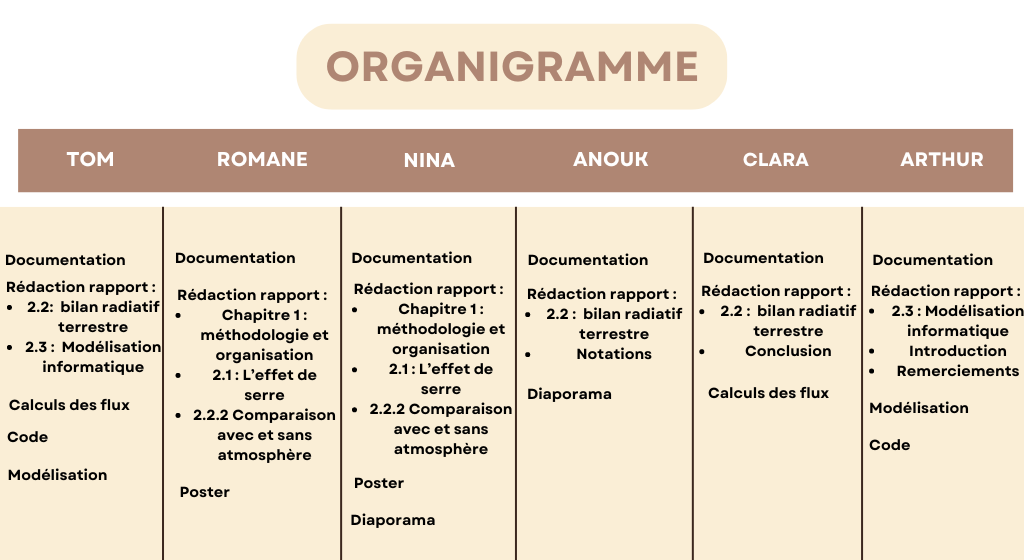
\includegraphics[scale=0.4]{Images/organigramme p6.png} 
\end{center}


%%% Travail réalisé et résultats

\chapter{Recherches, modèles et résultats sur l'effet de serre}

\section{L'effet de serre}

\subsection{Explication du phénomène de l'effet de serre}

	L'effet de serre est un processus naturel qui se produit 
avec le rayonnement entre la Terre et le Soleil. Tout d'abord, 
le Soleil émet un rayonnement vers la Terre, l'atmosphère 
laisse passer une partie de ce rayonnement solaire. 
Réchauffé, le corps terrestre, étant un CN, émet un rayonnement infrarouge. 
Ce flux est alors renvoyé vers l'atmosphère et une partie est absorbée par les gaz présents, appelés gaz à effet de serre. 
Le reste du flux est envoyé dans l'espace.\vspace{\baselineskip}

\begin{figure}[h]
    \begin{center}
    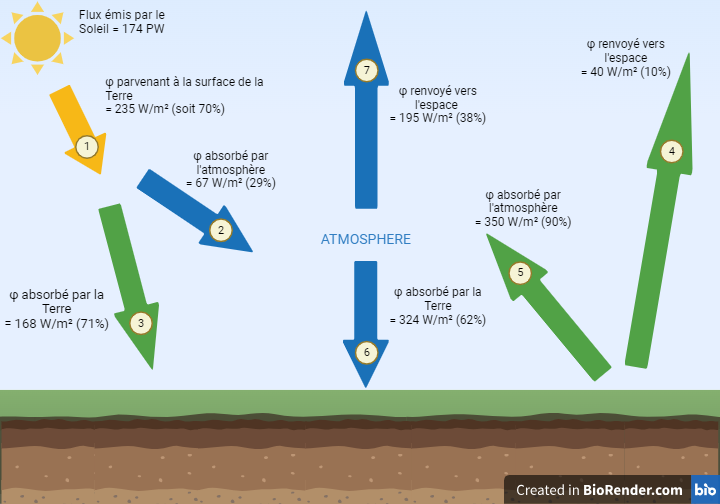
\includegraphics[scale=0.5]{Images/schemaflux.png}
    \figcaptionwithsource{Bilan radiatif terrestre}{\textit{Biorender}}{fig:figure1}
    \label{fig:figure1}
    \end{center} 
\end{figure}

Dans le but de comprendre ce phénomène plus en détail, nous allons maintenant expliciter 
différentes hypothèses. Premièrement nous allons considérer que les différents systèmes impliqués 
dans le phénomène d’effet de serre sont des CN. 

\subsection{Définition d'un corps noir et de l'émittance}
\noindent \textbf{Le corps noir}

\vspace{\baselineskip}
Un CN est un objet idéal qui permet d'évaluer le flux thermique maximum
que peut rayonner un corps, en fonction de sa température. Ainsi un CN 
va émettre autant de rayonnement qu'il en absorbe. On peut donc dire que son 
émittance $ \epsilon$  est égale à 1. \vspace{\baselineskip}

\noindent \textbf{L'émittance}
\vspace{\baselineskip}

\noindent L'émittance spectrale d'un CN est évaluée grâce à la loi de Planck :

\begin{center}
$M^{0}_{\lambda,T}= \frac{\pi C_1}{\lambda^5} \biggl(\exp(\frac{C_2}{\lambda T}) - 1\biggr)^{-1}$ \\
\end{center}

\noindent Et ainsi l'émittance totale d'un CN (en $W.m^{-2}$) est obtenue avec la formule suivante: \vspace{\baselineskip}

\hfil $M^{0}$ = $\int_{0}^{\infty} M^{0}_\lambda d\lambda$ = $\sigma T^{4}$ 

 \section{Bilan radiatif terrestre}
\par

\subsection{Bilan radiatif sans atmosphère} 

Dans un premier temps, il est important de comprendre que le seul échange thermique possible entre le Soleil
et la Terre est le rayonnement. Le Soleil émet des rayonnements dans le domaine visible et dans le domaine infrarouge. C'est un CN, c'est à dire qu'il absorbe tout le rayonnement qu'il reçoit et le ré-émet 
parfaitement. De plus , on peut dire que son émissivité est 
égale à 1 d'après les hypothèses du CN vues précédemment. Il suit donc la loi de Planck et son spectre d'émission en fonction de 
la longueur d'onde est le suivant : 

\begin{figure}[h]
    \begin{center}
    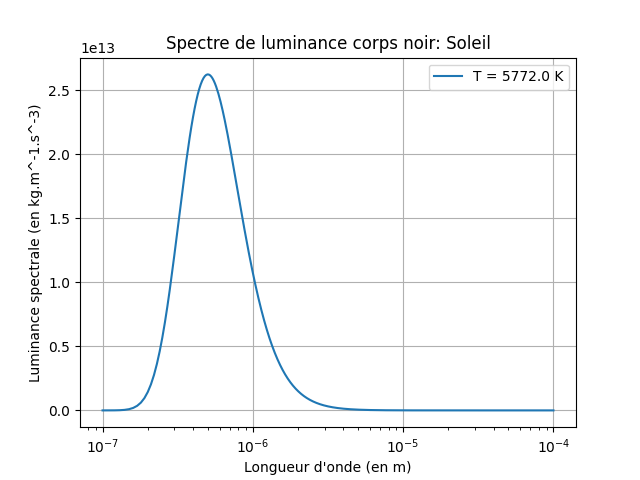
\includegraphics[scale=0.7]{Images/Spectre de luminance corps noir Soleil.png}
    \figcaptionwithsource{Spectre du Soleil, intensité du rayonnement solaire à $T_s$ = 5772 K}{\textit{Python 3.12}}{fig:figure1}
    \end{center} 
\end{figure}

\noindent On peut alors calculer ce qu'il émet de deux manières: \vspace{\baselineskip}

1. Avec l'expression du flux radiatif :
\begin{center}
$\Phi_{ray}$ = $\int_S \epsilon \sigma T^{4} dS$    
\end{center}
\begin{center}
$\Phi_{ray}$ = $\epsilon \sigma T^{4} S$    
\end{center}
avec T=5772 K la température du Soleil, l'émissivité 
$\epsilon = 1$ car le Soleil est un CN qui émet tous les rayonnements qu'il absorbe 
et sa surface $S=4\pi{R_S}^2$ 
\vspace{\baselineskip}

\noindent On trouve : \vspace{\baselineskip}
$\Phi_{ray}$ = $3,83.10^{26}$ W 

2. Numériquement : \vspace{\baselineskip}

En effet, évaluer le flux émit revient à calculer l'aire sous la courbe de son spectre d'émission.
Nous avons codé la fonction suivante \footnote{ \annexeref{Fonction luminance corps noir}} 
afin de calculer l'émittance d'un CN en fonction de la longueur d'onde. Nous avons ensuite intégré cette fonction sur la bande d'émission du Soleil et avons obtenu notre densité de flux suivante. \vspace{\baselineskip}

$\phi_{ray}$ = $6,29.10^7$ $W.m^{-2}$ 
$\Rightarrow$ $\Phi_{ray}$ = $4\pi{R_S}^2\phi_{ray}$ = $3,83.10^{26}$ W
\vspace{\baselineskip}

Cependant, comme le Soleil rayonne dans toutes les directions de l’espace, seul une petite partie de ce rayonnement arrive jusqu’à la surface de la Terre. 
La distance qui nous sépare du Soleil est un facteur à prendre en compte pour mesurer la quantité de rayonnements qui est reçu sur le sol terrestre. Ainsi   si la distance Soleil-Terre était plus petite, le flux radiatif  perçu par la Terre serait plus important.  \vspace{\baselineskip}

On calcule donc dans un premier temps la fraction p du rayonnement solaire qui parvient jusqu'à la Terre. 
On se place dans un disque ayant comme rayon la distance Soleil-Terre, puisque le Soleil émet dans toutes les directions.
La Terre ne reçoit qu'une petite partie de ce rayonnement sur la moitié de sa surface, puisque l'autre moitié de la Terre n'est pas éclairée (d'où le jour et la nuit). 

\begin{figure}[h]
    \begin{center}
    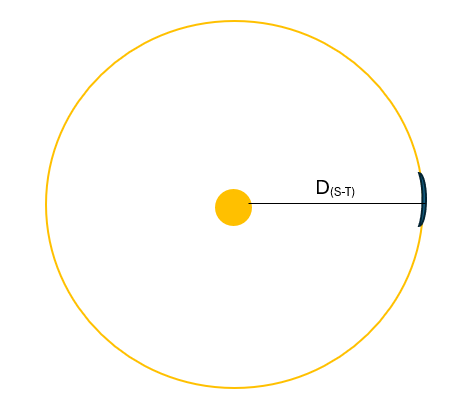
\includegraphics[scale=0.6]{Images/schemadistance.png}
    \figcaptionwithsource{Schéma du rayonnement solaire qui nous parvient}{\textit{Biorender}}{fig:figure1}
    \label{fig:figure1}
    \end{center} 
\end{figure}

De plus, $ D_{S-T}$ étant très grande devant le rayon de la Terre, on considère que la surface éclairée est modélisable en 2D par un disque de rayon $R_{T}$. La surface de la Terre vaut donc $\pi R_T^2$ . En 3D, la fraction p correspond à la proportion occupée par la surface de la Terre sur l'ensemble de la surface du disque jaune, soit $4\pi D_{S-T}^2$. Elle se calcule donc comme suit :

\begin{center}
$p$ = $\frac{\pi R_T^{2}}{4 \pi D_{(S-T)}^{2}}$ 
= $\Big( \frac{R_T}{2D_{(S-T)}} \Big)^2$ 
\end{center}

Ainsi le rayonnement solaire qui arrive au niveau de la surface de la Terre vaut: 

\begin{center}
$\Phi_{recu, Terre}$ = $\Phi_{ray} \times p = 174$ $PW$ = $1,74.10^{17}$ $W$   
\end{center}

\vspace{\baselineskip}

Enfin pour mesurer le flux absorbé par la Terre, il existe un second facteur de diminution qui s’explique par le phénomène d’albédo. En effet, 30 \% du rayonnement qui parvient jusqu’à la Terre est réfléchi par notre planète, donc seulement 70 \% du rayonnement est absorbé. 
\newline On peut alors calculer le flux absorbé par la Terre : 
\begin{center}
$\Phi_{abs,Terre}$ = $(1-\Bar{a_T}) \times \Phi_{recu, Terre}$    
\end{center}
\begin{center}
$\Phi_{abs,Terre}$ = $1,21.10^{17}$ $W$= $121$ $PW$  

\end{center}

    En divisant par la surface de la Terre, 
on obtient le flux surfacique absorbé par la Terre:
\begin{center}
$\phi_{abs,Terre}$ = $\frac {\Phi_{abs,Terre}}{4 \pi R_T^{2}}$
= 235 $W.m^{-2}$
\end{center}

\vspace{\baselineskip}

Retrouvons maintenant la température à sa surface.
On réalise un bilan thermique sur le système suivant : 
la Terre, sans son atmosphère.
\begin{center}
    Production = Échanges + Stockage 
\end{center} \vspace{\baselineskip}

Tout d'abord, la Terre produit de la chaleur grâce au processus de géothermie. En effet, l’activité radioactive au centre de la Terre qui correspond à la désintégration naturelle des atomes présents crée de la chaleur. Cependant, cette production thermique est négligeable par rapport à la chaleur apportée par le Soleil. On considère donc que le terme de production thermique dans notre bilan est nul. \vspace{\baselineskip}

De plus, à l’équilibre thermique, l’état est stationnaire, ce qui signifie que la température ne varie plus dans le temps et donc que notre système ne stocke pas d’énergie thermique. Le terme de stockage est nul, et on obtient alors : 

    \begin{center}
    Échanges = 0 $\Leftrightarrow \Phi_{emis} = \Phi_{absorbe}$
    \end{center}
    \vspace{\baselineskip}

On retrouve que la Terre sans son atmosphère est un CN, d’émissivité 1. En effet, tout le rayonnement qu’elle absorbe est réémis. On a donc d'après la loi de Planck :
\begin{center}
$\Phi_{emis,Terre}$ = $4 \pi R_T^{2} \sigma T^{4}$
\end{center} 

De plus, nous avons vu précédemment que
\begin{center}
$\Phi_{emis,Terre}$ = $\Phi_{abs,Terre}$  = 121 $PW$
\end{center} \vspace{\baselineskip}

On peut ainsi retrouver la température de la Terre : \vspace{\baselineskip}
\begin{center}
\boxed{ T = \sqrt[4]{\frac{\Phi_{abs,Terre}}{4 \pi R_T^{2} \sigma}} = 235 \text{ K} = -19^\circ \text{C} }
\end{center} \vspace{\baselineskip}

On comprend ici que sans atmosphère, la température terrestre
serait de -19°C. Nous pouvons en conclure que négliger l'atmosphère et les phénomènes qui s'y produisent
est absurde, puisque la température moyenne observée
sur Terre est bien supérieure, autour de 13,7 °C.

\subsection{Comparaison avec et sans atmosphère} 

\vspace{\baselineskip}
Nous allons donc par la suite prendre en compte l'atmosphère terrestre et l'effet de serre qui s'y produit et le comparer au cas sans atmosphère. Pour cela, nous allons confronter deux modèles : l'un  sans effet de serre et l'autre avec. Ce second modèle sera le plus simple possible, afin de réellement comprendre le phénomène d'effet de serre, c'est pourquoi nous avons considérer la température constante, quelle que soit l'altitude à laquelle nous nous situons dans l'atmosphère.

\vspace{\baselineskip}

Nous savons 
que l’atmosphère émet un rayonnement selon la loi de Planck qui dépend de la température. En effet, plus la température est élevée, plus le CN émet sur un large intervalle de longueur d'onde. 
On peut voir sur la figure suivante que le Soleil, autour de 6000K, émet au maximum pour une longueur d'onde dans le domaine visible, alors que pour la Terre à environ 300K, la longueur d'onde pour une émission maximum se trouve dans l'infrarouge.

\begin{figure}[h]
    \begin{center}
    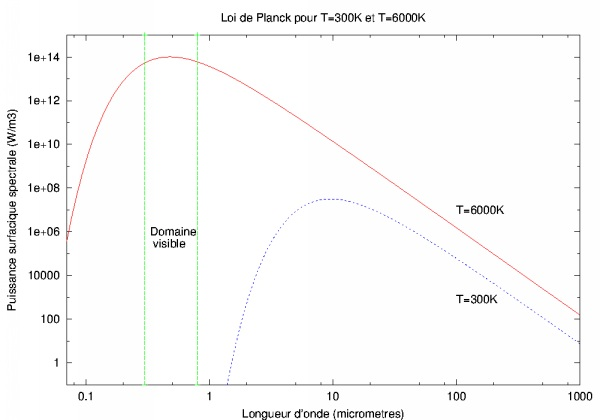
\includegraphics[scale=0.4]{Images/loiPlancksoleilterre.jpg}
    \figcaptionwithsource{Lois de Planck pour le Soleil et la Terre}
    {\url{https://planet-terre.ens-lyon.fr/}}{fig:figure1}
    \label{fig:figure1}
    \end{center} 
\end{figure}

Par conséquent, les températures de la surface de la Terre et de l’atmosphère étant égales dans ce 
premier modèle, ce qui est absorbé par l’atmosphère est ré-émis exactement de la même manière.
Ainsi, si l'on modélise ce phénomène afin d’obtenir le spectre au sommet de l’atmosphère, en utilisant le code de David Louapre, on obtient les courbes suivantes.

\begin{figure}[H]
    \begin{center}
    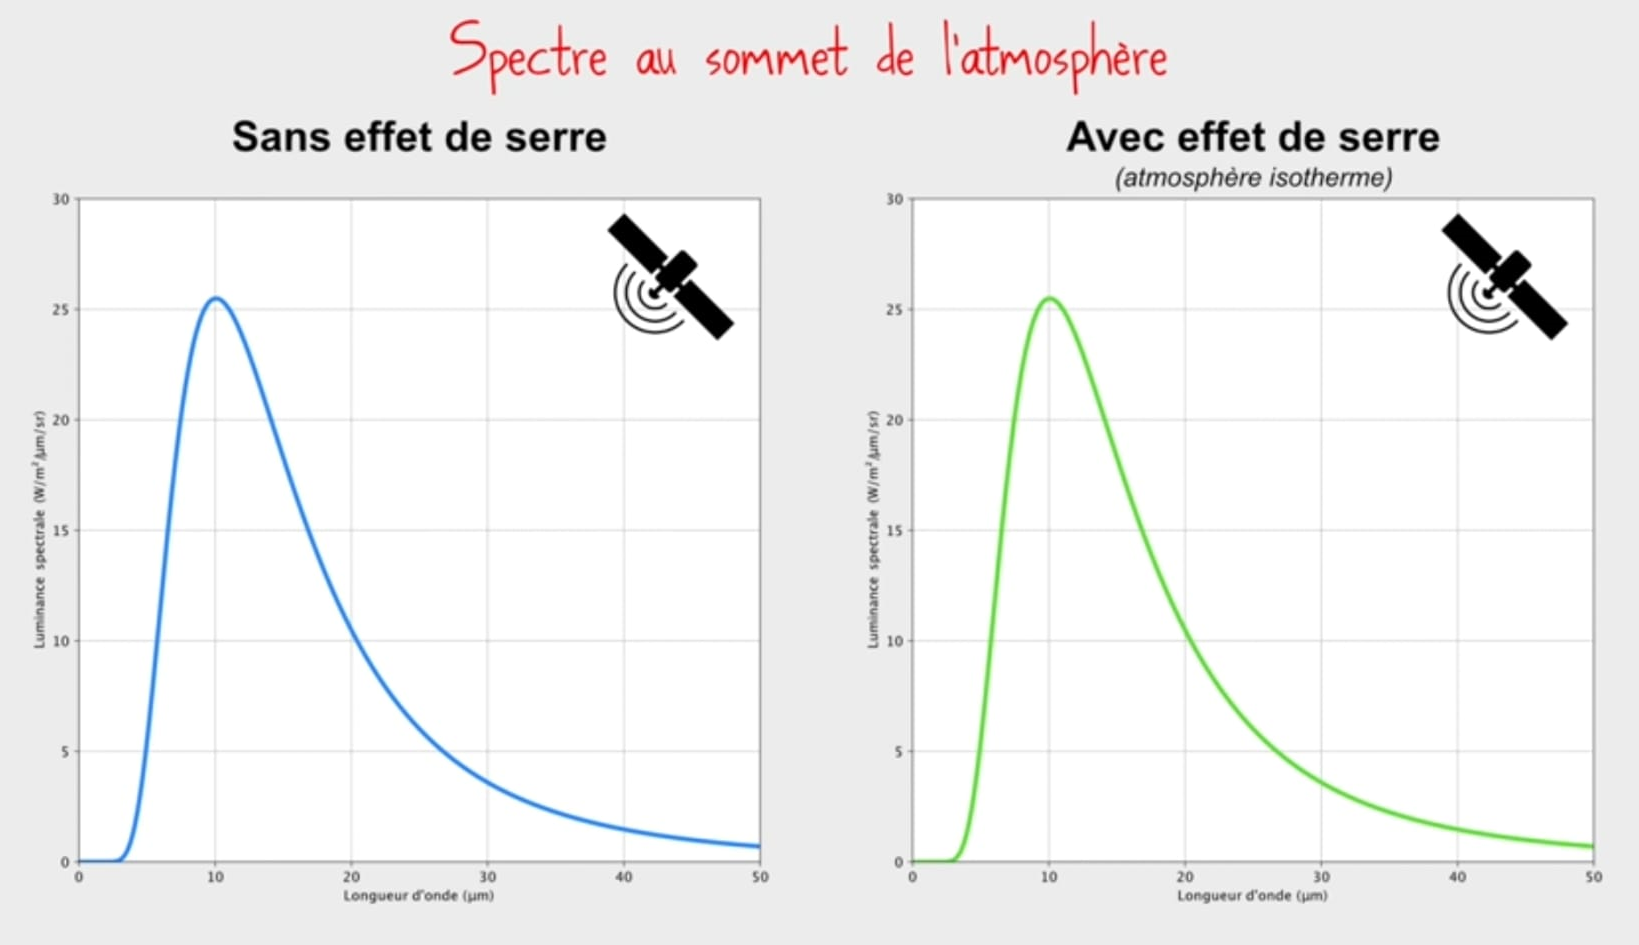
\includegraphics[scale=0.25]{Images/2modeles.png}
    \figcaptionwithsource{Spectre de rayonnement terrestre}{\url{https://www.youtube.com/watch?v=ewc8FBtEKPs}}{fig:figure1}
    \label{fig:figure1}
    \end{center} 
\end{figure}

En comparant ces deux courbes, nous pouvons voir que le spectre au sommet de l’atmosphère est le même avec ou sans la présence d'atmosphère et GES. La seule différence étant l’origine du 
rayonnement, qui ne provient que de la surface de la Terre pour celui sans effet de serre, mais de la surface de la Terre et des couches de l'atmosphère pour celui avec l’effet de serre. \vspace{\baselineskip}

Ainsi, si la température était uniforme dans l'atmosphère, nous n’aurions pas d’impact des gaz à effet de serre.
Or l’atmosphère est en réalité composée de plusieurs couches de température différentes. Chacune d’entre elles émet donc un rayonnement propre selon la loi de Planck. Ce qui est absorbé par l’atmosphère n’est donc pas ré-émis exactement de la même manière. La différence de température entre la surface de la Terre et les couches de l’atmosphère implique la présence d’un effet de serre, c'est à dire qu'une partie des rayonnements terrestres est absorbée par les gaz de l'atmosphère, les GES.

\subsection{Définition des GES et leur impact}

Un gaz à effet de serre est un gaz présent dans l'atmosphère qui 
absorbe une partie des rayonnements (rayons infrarouges) 
reçus par le Soleil. Ces gaz sont d'origine naturelle 
(vapeur d'eau, ozone...) et/ou anthropique 
(issues des activités humaines) comme par exemple le dioxyde 
de carbone ($CO_2$), le méthane ($CH_4$), le protoxyde d'azote
($N_2O$) et les gaz fluorés (HFC) \endnote{JEAN-MARC JANCOVICI, Article, \textit{"Quels sont les gaz à effet de serre ?"}, 01/08/2007: 
\\ \url{https://jancovici.com/changement-climatique/gaz-a-effet-de-serre-et-cycle-du-carbone/quels-sont-les-gaz-a-effet-de-serre-quels-sont-leurs-contribution-a-leffet-de-serre/} \vspace{\baselineskip}}. L'absorption du rayonnement de la Terre par les GES 
provoque un réchauffement qui se traduit ci-dessous par le spectre d'émission de la Terre vu depuis l'espace en présence de $CO_2$.

\begin{figure}[H]
    \begin{center}
    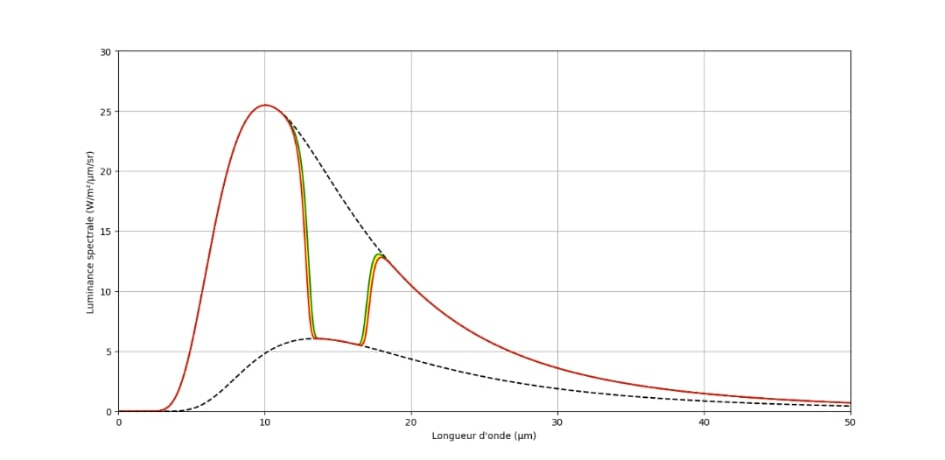
\includegraphics[scale=0.6]{Images/trou.png}
    \figcaptionwithsource{Spectre de rayonnement en présence de $CO_2$}{\url{https://www.youtube.com/watch?v=ewc8FBtEKPs}}{fig:figure1}
    \label{fig:figure1}
    \end{center} 
\end{figure}

La courbe en pointillés en bas correspond à la loi de Planck pour la température de 217 K, soit la température à 10 km d'altitude. Les courbes rouge et verte correspondent aux spectres de rayonnements observés depuis l'espace en présence de $CO_2$: en vert pour 0,028 $\%$ de $CO_2$ dans l'air, et en rouge pour 0,056 $\%$. Enfin la courbe en pointillés en haut correspond au spectre de rayonnement de la Terre sans atmosphère. \vspace{\baselineskip}

Bien que cette courbe reste une simplification, puisque l'absorption du $CO_2$ a été simplifiée en prenant en compte seulement la bande principale de son spectre, on remarque que la présence de $CO_2$, un GES, créé un trou dans le spectre de rayonnement de la Terre. L'aire sous la courbe du spectre de rayonnement terrestre est donc inférieure à ce qu'elle devrait être, la Terre n'est donc pas à l'équilibre thermique, puisqu'elle absorbe plus de rayonnement qu'elle n'en émet.
\vspace{\baselineskip}

Ainsi, la Terre va devoir émettre un plus grand rayonnement pour atteindre l'équilibre thermique, et donc se réchauffer. Ce phénomène créé un réchauffement global de la Terre permettant à la 
température moyenne de s'élever à 15 °C au lieu de -19 °C. 
	
% mettre schema flux radiatif

\subsection{Bilan radiatif avec effet de serre}

Désormais, considérons que l’atmosphère, en particulier un des gaz qui la compose, le $CO_2$, impacte les flux. 
En réalité, il s’agit de comprendre que lorsque le flux arrive sur les différentes molécules de $CO_2$, le flux est soit transmis, c’est-à-dire qu’il passe à travers les molécules, soit il est absorbé, soit il est réfléchit. Dans notre cas, on peut négliger la réflexion car elle est très petite devant les 2 autres pour un gaz. Nous avons donc, une partie du flux qui est alors transmise, et l’autre qui est absorbée, avec des coefficients respectifs $(\tau,\alpha) \in [0;1]^2$
\vspace{\baselineskip}

Ces coefficients d'absorption et de transmission sont propres à chaque molécule et dépendent de la longueur d’onde. Le fait que les coefficients dépendent des longueurs d’onde complexifie donc grandement le problème. Il faut utiliser la notion d'émittance pour calculer un flux que l'on pourra associer à ces coefficients.  

\begin{center}
$\phi$ =$\int_{\lambda} M^0_{\lambda,T} \, \mathrm{d}\lambda$
\end{center}

Avec cela, nous pouvons désormais calculer un flux en prenant en compte les interactions avec les molécules de l’atmosphère. La figure suivante présente les différents flux entre la Terre, le Soleil et l'atmosphère où chaque expression correspond au flux évoqué précédemment \footnote{Voir Figure 1}.  \vspace{\baselineskip}  

\begin{figure}[H]
    \begin{center}
    \includegraphics[scale=0.4]{Images/Schémafluxformules.png}
    \figcaptionwithsource{Quantification des flux de la figure 1}{\textit{Biorender}}{fig:figure1}
    \label{fig:figure1}
    \end{center} 
\end{figure}

\begin{center}
$\boxed{\sigma T_T^4$ = $\frac{1}{2} \int_{\lambda}^{} (1-\tau_{CO_2})M^{0}_{\lambda,T} \, \mathrm{d}\lambda 
                + \int_{\lambda}^{} \tau_{CO_2}E^{0}_{\lambda,T} \, \mathrm{d}\lambda \times (1-\Bar{a_T})
\ \ \ (BT)}$
\end{center}

    Avec $\sigma T_T^4$ le rayonnement émis par la Terre, considérée 
comme un CN, doit être égal à la somme des flux absorbés par la Terre pour être à  l'équilibre. Parmi ces flux, nous avons $\frac{1}{2} \int_{\lambda}^{} (1-\tau_{CO_2})M^{0}_{\lambda,T} \, \mathrm{d}\lambda$, qui provient du flux émis par la Terre qui a été absorbé par l'atmosphère. Une fois absorbé, il est réémis dans des proportions équivalentes vers l'espace et la Terre. De plus, il y a $\int_{\lambda}^{} \tau_{CO_2}E^{0}_{\lambda,T} \, \mathrm{d}\lambda \times (1-\Bar{a_T})$, qui provient de l'éclairement du Soleil transmis par l'atmosphère à la surface de la Terre. Seulement 70 $\%$ de ce flux est absorbé par la Terre, dû au phénomène de l'albédo. \vspace{\baselineskip}

L’objectif est de quantifier les différentes flèches, afin d’utiliser le bilan thermique et de déterminer la température de la Terre en considérant les effets des gaz de l’atmosphère. Comme nous avons dit ci-dessus, le coefficient d'absorption, $\alpha_{CO_2} = 1 - \tau_{CO_2}(\lambda)$, dépend de la longueur d’onde, puisque les gaz à effet de serre n'absorbent pas à toutes les longueurs d'onde de la même manière. \vspace{\baselineskip}

L'absorption du $CO_2$ à une certaine altitude correspond à son coefficient d'absorption à la longueur d'onde considérée $k_{abs}(\lambda)$, multiplié par la densité particulaire volumique de $CO_2$ présent à cette altitude de l'atmosphère $n_{CO2}(z)$, soit $k_{abs}(\lambda) \times n_{CO2}(z)$. L'absorption totale pour une longueur d'onde donnée correspond alors à la somme de cette absorption pour toutes les altitudes, d'où : 
\begin{center}
    $1-\tau_{CO2}(\lambda)$ = $\int_{0}^{h_{max}} k_{abs}(\lambda) \times n_{CO2}(z) \, \mathrm{d}z$
\end{center}

\subsection{Modélisation de l'atmosphère en fonction de l'altitude}

La température dans l'atmosphère n'est pas isotherme, elle varie selon l'altitude. Pour déterminer la densité moculéculaire dans l'atmosphère, il nous faut des profils de température selon l'altitude. Nous avons fait le choix d'utiliser le modèle atmosphère standard dit ISA \endnote{Article, \textit{"International Standard Atmosphere"}, 30/05/2024 \\
\url{https://en.wikipedia.org/wiki/International_Standard_Atmosphere}} 
Ainsi, nous obtenons les profils de température (en K) suivant les couches atmosphériques selon l'altitude (en m): \vspace{\baselineskip}

T(z) =
\begin{cases}
-6,5.10^{-3}z + 288,15
&, \ 0  \leq z < z_{trop} \ = \ $1,1.10^4$ $m$\\ 
216,65 
&, \ z_{trop} \leq z < z_{strat1} \ = \ $2,0.10^4$ $m$ \\ 
1,0.10^{-3}(z - z_{strat1}) + 216,65
&, \ z_{strat1} \leq z < z_{strat2} \ = \ $4,7.10^4$ $m$ \\
2.8.10^{-3}(z - z_{strat2}) + 228,65
&, \ z_{strat2} \leq z \leq z_{meso} \ = \ $5,1.10^4$ $m$ \\
\end{cases}

\begin{figure}[H]
    \begin{center}
    \includegraphics[scale=0.65]{Images/Température.png}
    \figcaptionwithsource{Profil de température atmosphérique en fonction de l'altitude}{\textit{Python 3.12}}{fig:figure1}
    \label{fig:figure1}
    \end{center} 
\end{figure}
\vspace{\baselineskip}

Grâce à ces profils de température, nous allons pouvoir dans un premier temps exprimer la pression en fonction de l'altitude. Pour cela, nous pouvons commencer par le cas de la température uniforme entre 11 km et 20 km. En utilisant le principe fondamental de la statique des fluides et le modèle des gaz parfaits on a:

\begin{center}
    $\frac{dP}{dz} = -\rho g = \frac{dP}{dz} = -\frac{PM}{RT}g
    \Leftrightarrow \frac{dP}{P}$= $-\frac{gM}{RT} dz
    \Rightarrow P(z)= C\times e^{-\frac{gM}{RT} z }$
\end{center}

Grâce aux conditions initiales du modèle, et en imposant une contrainte de continuité, il est possible de calculer C car nous connaissons la pression de base de la troposphère..

\begin{center}
     $P(z_i)  = C\times e^{-\frac{gM}{RT} z_i }$
\end{center}

\begin{center}
     $C = \frac{P(z_i)}{e^{-\frac{gM}{RT} z_i}}$
\end{center}

\begin{center}
     ${P(z)} = {P(z_{trop})}{e^{-\frac{gM}{RT} (z - z_{trop})}}$
\end{center}

    Désormais, pour trouver la pression dans le cas général, on
utilise une formule plus générale:
\begin{center}
$T(z)=az+b$
\end{center}

On peut calculer la pression en fonction de l'altitude, en utilisant à nouveau le principe fondamental de la statique des fluides.
\begin{center}
     $\frac{dP}{dz}$ = $\frac{-{P} Mg}{R(az+b)}
     \Leftrightarrow \frac{dP}{P}$ = $\frac{dz}{(az+b)} \times \frac{- Mg}{R}
     \Rightarrow \ln(P)=\frac{-Mg}{Ra} \ln(az+b)+K$
\end{center}

\begin{center}
     $\Leftrightarrow P(z) = e^{\frac{-Mg}{Ra}\ln(az+b)} \times e^k =(az+b)^{\frac{-Mg}{Ra}} \times C \ , \ C = e^{K}$
\end{center}

On peut déterminer la constante C grâce aux conditions limites imposées par la continuité de la pression les transition de nos modèles atmosphériques en $z = z_{trop}$ et $z = z_{strat1}$. On notera par $P(z_i)$ et $z_i$, l'altitude et la pression de base de la portion du modèle \footnote{Par exemple pour la stratosphère, on aura un $z_i = 0$ et $P_0 = P_{mer} = 10^5 \ Pa$}.

\begin{center}
$P(z_i) = (a{z_i}+b)^{\frac{-Mg}{Ra}} \times C
\Rightarrow C= \frac{P(z_i)}{((a{z_i}+b))^{\frac{-Mg}{Ra}}}$
\end{center}

\begin{center}
$\therefore \ P(z) = (az+b)^{\frac{-Mg}{Ra}} \times \frac{P(z_i)}{(a{z_i}+b)^{\frac{-Mg}{Ra}}} {P(z_i)} \bigl(\frac{az+b}{a{z_i}+b}\bigr) ^ {\frac{-Mg}{Ra}} = {P(z_i)} \bigl(\frac{T(z)}{T(z_i)}\bigr) ^ {\frac{-Mg}{Ra}}$
\end{center}
\vspace{\baselineskip}

On peut tracer la courbe de la pression en fonction de l'altitude :
\begin{figure}[H]
    \begin{center}
    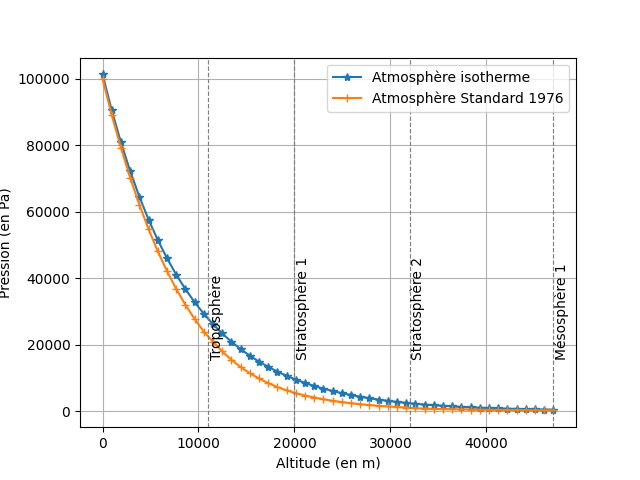
\includegraphics[scale=0.6]{Images/Pression.png}
    \figcaptionwithsource{Profil de la pression en fonction de l'altitude}{\textit{Python 3.12}}{fig:figure1}
    \label{fig:figure1}
    \end{center} 
\end{figure} 
\vspace{\baselineskip}

% P(z) = 
% \begin{cases}
% {P(z_i)} \left(\frac{T(z)}{T(z_i)}\right) ^ {\frac{-Mg}{Ra}}
% &, \ $z \in [0;z_{trop}[\cup[z_{strat1};z_{meso}[$ \\

% {P(z_{trop})}{e^{-\frac{gM}{RT} (z - z_{trop})}}
% &, \ $z \in [z_{trop};z_{strat1}[$
% \end{cases} \vspace{\baselineskip}

D'après la Loi des Gaz Parfaits on peut écrire :
\begin{center}
    $PV = Nk_BT$
    $\Leftrightarrow$ $\frac{N}{V}= \frac{P}{k_BT}$
    $\Leftrightarrow$ $n(z)= \frac{P(z)}{k_BT} $
\end{center}

Ainsi on a : 
n(z) =
\begin{cases}
\frac{{P(z_i)}\big(\frac{T(z)}{T({z_i})}\bigl)^{\frac{-Mg}{Ra(z)}}}{{k_B}{T(z)}}
&, \ $z \in [0;z_{trop}[\cup[z_{strat1};z_{meso}[$ \\

\frac{ P(z_i) e^{-\frac{gM}{RT} (z-z_{trop}) }}{{k_B}T}
&, \ $z \in [z_{trop};z_{strat1}[$
\end{cases}

\begin{figure}[h]
    \begin{center}
    \includegraphics[scale=0.6]{Images/Densité particulaire volumique.png}
    \figcaptionwithsource{Profil de la densité particulaire volumique de l'air en fonction de l'altitude}{\textit{Python 3.12}}{fig:figure1}
    \label{fig:figure1}
    \end{center} 
\end{figure}

% Perso je l'aurais écrirt en rajoutant qq petits trucs comme ça (en-dessous)
On remarque que le profil de la DPV tend vers 0 à partir de la couche de la mésosphère. En effet, cela s'explique par le fait que la pression tende elle aussi vers 0, puisque la colonne d'air surfacique voit sa hauteur diminuer et donc sa force réduire. Ainsi, on peut considérer que cette DPV sera négligeable et n'aura aucun impact sur le coefficient de la transmitance au-delà de la mésosphère. Ceci conforte notre choix d'avoir opté pour un profil d'atmosphère s'étendant seulement jusqu'à la mésosphère.
\vspace{\baselineskip}

En ayant le profil de la densité moléculaire volumique, on peut ainsi à l'aide du programme Python \footnote{Voir \ref{subsubsec:Modèle 3 info}} calculer (1-$\tau_{CO2}$), et ainsi calculer l'intégralité des flèches.
En reprenant l'équation bilan déterminée plus haut (BT), on pourra calculer numériquement la température de la Terre.

\section{Modélisation informatique et compilation}

    Maintenant que le phénomène d'effet de serre a été expliqué
physiquement et mis en équation mathématiquement, il reste encore à le transcrire informatiquement. Pour cela nous reprendrons les modèles décrits dans la partie précédente et tenterons de quantifier les divers flux de rayonnements impliqués dans le bilan thermique terrestre. 

\subsection{Récupération et traitement des données initiales}

    Avant toute chose, il a été nécessaire de se fixer
un point de départ à partir duquel nous entamerions l'implémentation de nos modèles informatiquement. Dans notre cas nous avons fait le choix de creuser jusqu'à constitution-même de notre base de donnée regroupant les caractéristiques physiques du $CO_2$. \vspace{\baselineskip}

    Plus précisément, pour mener nos calculs nous aurons besoins d'un 
ensemble de données initial: la transmittance du $CO_2$ et sa longueur d'onde associée. Nous avons stocké ces deux grandeurs sous forme d'un tableau à 2 colonnes dans un fichier, afin que cela soit facilement manipulable en Python. \vspace{\baselineskip}

    Sinon, pour en revenir à la démarche de construction de nos
modèle, nous avons parcouru 3 méthodes de traitement de données initiales différentes. La première portait sur une base de donnée assez rudimentaire et offrant peu de paramètres. Ensuite pour les méthodes suivantes, nous avons utilisé une même base de donnée plus complexe mais davantage polyvalente. La différence entre ces deux derniers modèles résidait dans la considération d'une atmosphère très simplifiée d'une part, et d'une atmosphère plus réaliste.

\subsubsection{Modèle 1: NIST}

    La base de données NIST
\endnote{COBLENTZ SOCIETYCollection (C) 2018 copyright by the U.S. Secretary of Commerce on behalf of the United States of America. All rights reserved, COBLENTZ NO. 8753, 1964 \vspace{\baselineskip}}, qui nous a permis d'extraire nos premières données liant la transmittance du dioxyde de carbone en fonction de la longueur d'onde. \vspace{\baselineskip}

    Cela nous a permis de réaliser nos premiers calculs de flux en
considérant l'impact de l'effet de serre dû au $CO_2$. Cependant cette base de donnée présentait de trop nombreux inconvénients pour une poursuite plus approfondie de notre étude: \newline
    \par - manque de transparence sur l'obtention des données 
    \par - peu de portabilité si l'on souhaite changer de GES
    \par - aucune maniabilité de la transmittance avec d'autres variables de notre modèle
    \par - impossibilité d'introduire une dépendance sur la quantité de $CO_2$ de l'atmosphère
    \par - plage de données de longueur d'onde non-ajustable

\subsubsection{Modèle 2: HITRAN, atmosphère simplifiée}

    La base de données HITRAN \footnote{Acronyme pour High
Resolution Transmission} a été une découverte très intéressante puisqu'elle est venue combler l'ensemble des défauts listés ci-dessus pour la base de donnée NIST. En effet, avec HITRAN nous avons eu accès à un module directement intégré à Python. Son utilisation bien que complexe, car faisant appel à des notions de physique avancées, s'est faite naturellement grâce à une API très bien documentée \endnote{ROMAN V.KOCHANOV, Documentation, "HITRAN Application Programming Interface (HAPI)", 14/04/2019: \url{https://hitran.org/static/hapi/hapi_manual.pdf} \vspace{\baselineskip}}. \vspace{\baselineskip}

    D'une part, nous avons travaillé avec une atmosphère
parfaitement isotherme, dont la température s'établissait à 296 K, soit la température moyenne de la Terre. Il a donc été simple de récupérer l'ensemble des données initiales, puisque qu'il était directement issu des fonctionnalités basiques du module \texttt{hapi} \footnote{\annexeref{Annexe Hitran z constant}}

\subsubsection{Modèle 3: HITRAN, atmosphère complexe}\label{subsubsec:Modèle 3 info}

    D'autre part, nous avons travaillé avec une atmosphère basée
sur le modèle ISA, où la température, ainsi que d'autres paramètres comme la pression et la DPV dépendaient tous de l'altitude atmosphérique. \vspace{\baselineskip}

   En parvenant à définir une fonction de densité particulaire
volumique par unité d'altitude, il a donc été possible de déterminer par nous-même un taux de transmission du $CO_2$ qui prend en compte sa répartition atmosphérique. Pour ce faire, nous avons intégré la fonction de DPV par rapport à l'altitude de 0 à $z_{meso}$ de notre à pouvoir obtenir la transmittance en multipliant par $k_{abs}$ puis en passant au complémentaire.

\subsection{Subtilités et techniques d'implémentation}

    Une fois les données de longueur d'onde et de transmittance du
$CO_2$ collectées dans un fichier, la physique et les calculs de flux sont indépendants de la base de donnée initiale. Voici donc le protocole général que nous avons adopté pour quantifier les différents flux impliqués dans l'équation de bilan thermique de la Terre.

\begin{center}
$\sigma T_T^4$ = $\frac{1}{2} \int_{\lambda}^{} (1-\tau_{CO_2})M^{0}_{\lambda,T} \, \mathrm{d}\lambda 
                + \bar{a_T} \int_{\lambda}^{} \tau_{CO_2}E^{0}_{\lambda,T} \, \mathrm{d}\lambda$
\ \ \ (BT)
\end{center}

\subsubsection{Implémentation de variables fonctionnelles au sens mathématique}

    \indent Un point fondamental dans ce projet est la nécessité de
manipuler des fonctions en Python dont la sortie soit elle-même de type \texttt{<function>}. L'intérêt de cette méthode est qu'une fois cette sortie récupérée et stockée dans une variable, nous pouvons manipuler cette nouvelle variable comme s'il s'agissait elle-même d'une fonction au sens mathématique. Cela signifie que l'on peut stocker des fonctions mathématiques, qui soient à la fois évaluables et intégrables, ce qui facilite énormément les manipulations lorsque l'on enchaîne les calculs divers. \vspace{\baselineskip}

    \indent Pour ce faire, rien de plus simple, il suffit de suivre le
schéma d'algorithmique suivant, qui consiste en une imbrication de deux fonctions Python. La première, celle imbriquée, retourne la valeur correspondant à l'image par la fonction en un point donné, tandis que la deuxième retourne l'ensemble des résultats des valeurs prises par la première. \vspace{\baselineskip}

    \indent Pour davantage de clarté regardons l'implémentation au
travers de l'exemple ci-dessous, dont l'objectif est de de retourner un objet de type \texttt{<function>}, qui soit le produit de deux objets de type \texttt{<function>} en entrée.

\begin{figure}[h]
    \begin{center}
    \includegraphics[scale=0.3]{Images/Exemple fonction mathématique Python.png}
    \figcaptionwithsource{Exemple de mécanisme de développement de fonction mathématique en Python}{\textit{Python 3.12}}{fig:figure1}
    \label{fig:figure1}
    \end{center} 
\end{figure}

    \indent Cette fonction \texttt{produit_de_fonctions} nous a
d'ailleurs été utile lorsqu'il a fallu intégrer un terme, étant lui-même composé d'un produit de deux objets de type \texttt{<function>}. 
Ça a par exemple été le cas pour les deux intégrandes dans l'expression des intégrales de (BT), où à la fois l'émittance ainsi que le taux de $CO_2$ étaient des fonctions de la longueur d'onde.

\subsubsection{Continuité mathématique et physique contre réalité informatique}

    L'utilisation d'un tableau de données correspond à une approche
discrète du problème, tandis que l'opération d'intégration présente dans (BT) requiert une intégrande qui soit continue. Notons que les méthodes d'intégration par discrétisation comme l'intégrale de Riemman ou la méthode des trapèzes seraient ici bien trop complexe à implémanter pour les raisons suivantes: \newline
    \par - intervalle entre deux longueur d'onde pas toujours constant
    \par - accumulation d'incertitudes de calcul
    \par - obligation de mixer des fonctions continues et des relations discrètes dans des intégrales
    \vspace{\baselineskip}

    De ce fait, il a fallu trouver une méthode pour rendre continue la
relation entre $\lambda$ et $\tau_{CO_2}$. Notre objectif pouvait se traduire mathématiquement par un problème d'interpolation à partir de séries statistiques, dont la taille était de l'ordre de $n=10^6$ éléments. De ce fait il était hors de question de trouver un polynôme avec un tel degré passant par tous nos points, nous avons donc opté pour une interpolation linéaire sur $\big((\lambda;\tau_{CO_2})_i\big)_{i \in [\![1;n]\!]}$.
\vspace{\baselineskip}

    Pour ce faire, nous avons utilisé le module \texttt{scipy}
\endnote{Pauli Virtanen, Ralf Gommers, Travis E. Oliphant, Matt Haberland, Tyler Reddy, David Cournapeau, Evgeni Burovski, Pearu Peterson, Warren Weckesser, Jonathan Bright, Stéfan J. van der Walt, Matthew Brett, Joshua Wilson, K. Jarrod Millman, Nikolay Mayorov, Andrew R. J. Nelson, Eric Jones, Robert Kern, Eric Larson, CJ Carey, İlhan Polat, Yu Feng, Eric W. Moore, Jake VanderPlas, Denis Laxalde, Josef Perktold, Robert Cimrman, Ian Henriksen, E.A. Quintero, Charles R Harris, Anne M. Archibald, Antônio H. Ribeiro, Fabian Pedregosa, Paul van Mulbregt, and SciPy 1.0 Contributors. (2020) SciPy 1.0: Fundamental Algorithms for Scientific Computing in Python. Nature Methods, 17(3), 261-272. \vspace{\baselineskip}} 
qui propose un grand nombre de fonctionnalités mathématiques très sophistiquées, et en particulier une qui répond exactement à notre problème d'interpolation 
\endnote{TYLER REDDY and RALF GOMMERS, Documentation, 02/03/2024: \url{https://docs.scipy.org/doc/scipy/reference/generated/scipy.interpolate.interp1d.html#scipy.interpolate.interp1d} \vspace{\baselineskip}}
: \ \texttt{class scipy.interpolate.interp1d(x, y, kind = 'linear', axis = -1, copy = True, bounds_error = None, fill_value = nan, \\ assume_sorted = False)} \vspace{\baselineskip}

    \indent Nous avons donc interpolé
\footnote{\annexeref{Annexe Interpolation}} entre chaque point selon un modèle linéaire, sur une certaine plage de donnée s'étendant de $1$ $\mu m$ à $20$ $\mu m$. En dehors de cette plage les valeurs, un appel à la fonction en l'un de ses points, renvoie automatiquement une valeur de 1 ou 0, pour respectivement la transmittance et l'absorbance du $CO_2$: il s'agit du rôle du paramètre \texttt{fill_value}. 

\begin{figure}[H]
    \begin{center}
    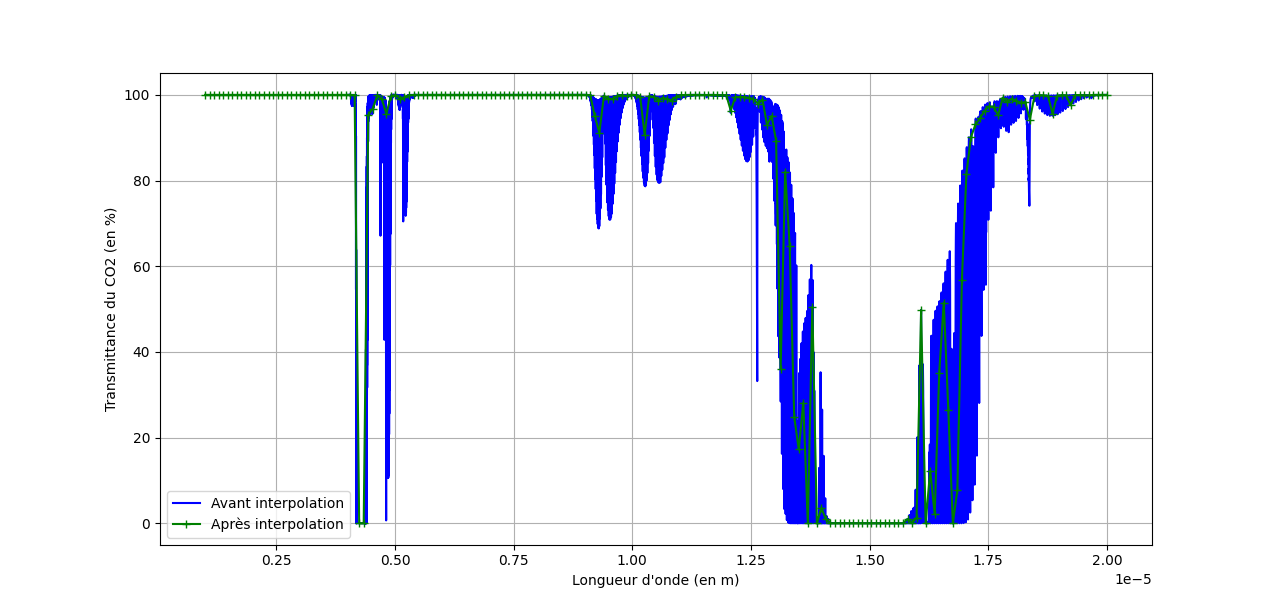
\includegraphics[scale=0.55]{Images/Taux transmission CO2 1.png}
    \figcaptionwithsource{Graphe de la courbe d'interpolation de la fonction transmittance}{\textit{Python 3.12}}{fig:figure1}
    \label{fig:figure1}
    \end{center} 
\end{figure}

\begin{figure}[H]
    \begin{center}
    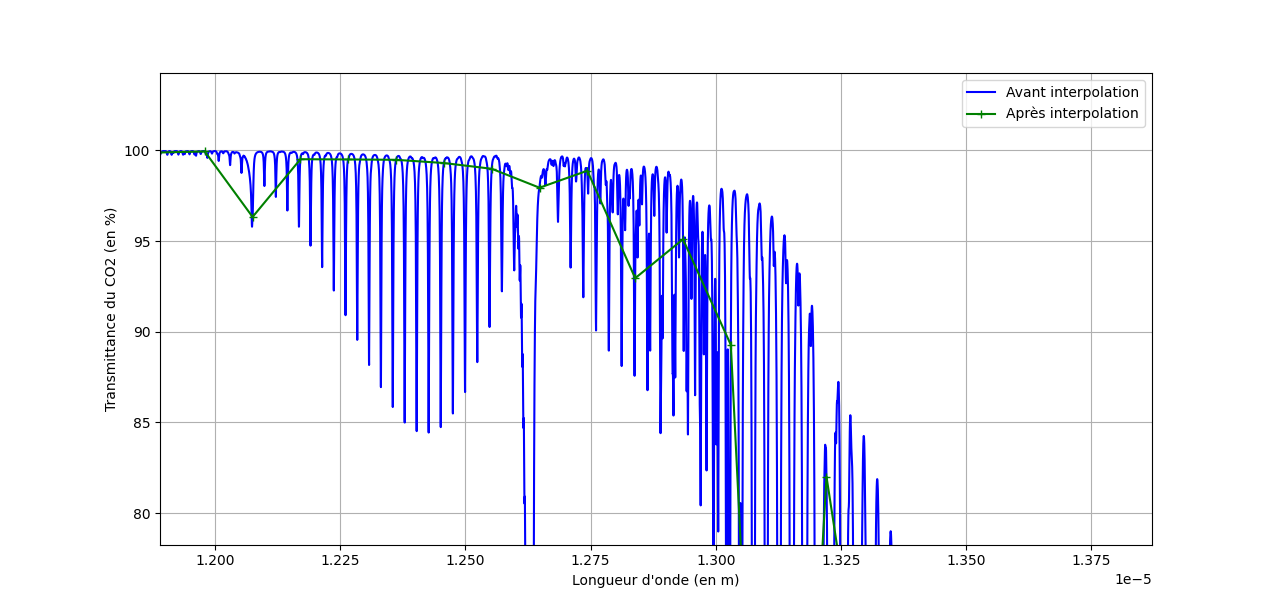
\includegraphics[scale=0.55]{Images/Taux transmission CO2 2.png}
    \figcaptionwithsource{Zoom sur les oscillations des données brutes et l'interpolation linéaire}{\textit{Python 3.12}}{fig:figure1}
    \label{fig:figure1}
    \end{center} 
\end{figure}

    Sur ces graphiques, il est essentiel de noter que la courbe
obtenue avant interpolation est un lissage réalisé par Python d'une grande multitude de points \footnote{Il y a près de 200 000 points au total dans la base donnée sur la seule plage considérée} obtenus via la base de donnée. En réalité la courbe d'interpolation est continue, bien que tracée volontairement avec un faible nombre de points dans le but de mettre en avant l'aspect linéaire.

\subsubsection{Fonctions définies par morceau}

    Le développement du modèle 3 est basé sur un découpage de
l'atmosphère en couches distinctes, selon l'évolution de la température en fonction de l'altitude. Pour évaluer les quantités, il a donc naturellement était nécessaire de mettre en place des fonctions définies par morceau, c'est-à-dire des fonctions dont l'expression dépend de l'intervalle ou de point traité. Grâce au module \texttt{numpy} \endnote{Harris, C.R., Millman, K.J., van der Walt, S.J. et al. Array programming with NumPy.} il a été possible de définir un tel concept informatique avec la fonction suivante: \texttt{numpy.piecewise(x, condlist, funclist)} \vspace{\baselineskip}

    Cette technique a notamment été utilisée lors de l'implémentation
de nos fonctions sur les caractéristiques physiques atmosphériques: les coefficients divers \footnote{\annexeref{Annexe Fonction  coefficients}}, la pression \footnote{\annexeref{Annexe Fonction pression}}, la température \footnote{\annexeref{Annexe Fonction température}} et la DPV \footnote{\annexeref{Annexe Fonction DPV}}.
    
\subsection{Calculs de flux et mise en pratique: difficultés et limites}

    Jusqu'à présent au niveau informatique, la modélisation consistait
à un ensemble de fonctions et de tests, mais aucun résultat significatif n'en avait encore été tiré. Et c'est bien là tout le problème, car en voulant construire un modèle complexe d'atmosphère, nous avons cru pouvoir conclure en calculant les flux comme pour les modèles 1 et 2. Cependant, au moment de passer à l'application de notre modèle d'atmosphère sur les flux, nous nous sommes retrouvés confrontés à un souci: la définition de la transmittance du $CO_2$ telle que définie précédemment dans le modèle 3, ne correspond à aucune réalité physique. \vspace{\baselineskip}

    La raison réside dans le fait qu'en réalisant les calculs pour
parvenir à $\tau_{CO_2}$, nous obtenons des valeurs comprises entre 0 et 1, mais à partir d'une certaine longueur d'onde, ces dernières divergent complètement dans les valeurs négatives extrêmes. Nous avons tant bien que mal tenté de résoudre ce confit, mais il s'avère que nous ne sommes parvenu à comprendre la source de notre erreur. D'autant plus qu'en tentant de vérifier la cohérence de notre intégrale avec une valeur moyenne, nous sommes avons retrouvé une valeur cohérente de la masse volumique de l'air, ce qui nous trouble d'autant plus. \vspace{\baselineskip}

$I = \frac{1}{z_{meso}}\int_{0}^{z_{meso}}n_{CO2}(z) \, \mathrm{d}z = 2,5.10^{25} \ molec.m^{-3} \Rightarrow \frac{IM(air)}{N_A} \approx 1.204.10^3 \ g.L^{-1}$ 
\vspace{\baselineskip}

    Le fait de ne pas parvenir à comparer les résultats de nos
différents modèles est décevant, surtout que nous avions investi une grande partie de notre recherche sur ce dernier modèle. Notre travail n'a pas été réalisé en vain, puisqu'il nous a permis de mieux appréhender le système atmosphérique et de proposer une sérieuse piste d'amélioration du modèle par David Louapre. Ce dernier se base sur un calcul du flux couche par couche, qui calcule le flux avec un certain défini par un paramètre de delta d'altitude, mais qui se prend moins en compte, du moins avec des modèles moins complexes, les paramètres atmosphériques. Une adaptation de son code avec nos outils pourrait donc offrir une représentation encore plus proche de la réalité physique.
    
\chapter*{Conclusion et perspectives}
\addcontentsline{toc}{chapter}{Conclusion et perspectives}

    Au cours de ce projet, nous avons modélisé l'atmosphère terrestre
de 3 manières différentes. Premièrement, nous n'avons pris en compte aucune action de l'effet de serre. Dans un second temps, nous avons considéré l'impact du $CO_2$, le principal GES en terme d'influence sur le bilan thermique, dans le cas d'une atmosphère isotherme. Enfin, nous avons pris en compte l'action du $CO_2$ pour une température variable selon l'altitude et d'autres paramètres physiques atmosphériques. \vspace{\baselineskip}

    Afin de comprendre concrètement l'impact des GES
sur la température de la Terre, nous avons modélisé en Python ces 3 cas. Ces modèles nous on permis de quantifier les flux absorbés, réfléchis et émis par le Soleil, la Terre et l'atmosphère.
Les résultats diffèrent complètement entre les modèles 1 et 2, puisque que la différence de température estimée était de presque 20 °C.
\vspace{\baselineskip}

    Grâce à ce projet, nous avons pu comprendre l'effet de serre. Nous
avons également pu approfondir par nous-même le cours de P8 de M. Yon vu en début de semestre sur les transferts thermiques. Pour une partie d'entre nous souhaitant faire GE l'année prochaine, c'est un thème qui nous intéresse et que nous serons amenés à approfondir dans le cycle ingénieur. \vspace{\baselineskip}

    Ce projet a également été enrichissant sur le plan technique,
puisque la majorité d'entre nous n'avait jamais utilisé les outils que sont \LaTeX et Github pour travailler à plusieurs et rédiger un rapport. Nous avons aussi appris à rechercher, exploiter et trier des informations scientifiques. \vspace{\baselineskip}

    Le fait que nous ne soyons parvenus à mener notre dernier modèle à
bout, nous a énormément déçu sur le moment. Avoir des ressources en temps limitées a aussi palier à la compréhension de nos erreurs quant à ce problème. Malgré tout, nous ne cherchons pas d'excuse, et garderons à l'esprit le principe suivant qui nous fera tous grandir pour le futur de notre carrière de scientifiques: une théorie solide et révisée sur le papier requiert malgré tout des ajustement parfois imprévus lors de l'application dans un cas pratique. \vspace{\baselineskip}

    Enfin, il a aussi été fructueux de collaborer entre membres du
groupe, certes issus de l'ingénierie, mais avec des compétences et appétences plus prononcées pour certains domaines que d'autres. De ce fait, cela a permis à chacun de se dédier à un aspect précis du projet, que ce soit dans la partie physique, mathématique ou informatique. L'apport et le partage des savoirs de chacun ont donc été très riches. Cela nous a permis d'aboutir à un projet que nous sommes tous à la fois fiers d'avoir réalisé et présenté. \vspace{\baselineskip}

%%% Table des figures

\newpage
\addcontentsline{toc}{chapter}{Table des figures}
\pagenumbering{gooble}
\setlength{\cftbeforeloftitleskip}{0pt}
\listoffigures


%%% Bibliographie

\newpage

\renewcommand{\notesname}{} % Laisse vide le titre de la section
\chapter*{Bibliographie}
\addcontentsline{toc}{chapter}{Bibliographie}
\renewcommand{\theendnote}{\fumprint{\value{endnote}}}
\makeatletter
\renewcommand{\enoteheading}{\par\vspace{1 em}}
\renewcommand{\theenmark}{\makebox[1 em][r]{\hfil\@theenmark\hfil}}
\renewcommand{\enoteformat}{\parindent = 2 em
  							\leftskip = 0.5 em
  							[\theenmark]\enspace\ignorespaces}							
\makeatother
\theendnotes

%%% Annexes

\newpage
\chapter*{Annexes}
\addcontentsline{toc}{chapter}{Annexes}

\newcounter{annexe}
\renewcommand{\theannexe}{\Alph{annexe}}
\newcommand{\annexe}[2]{
    \refstepcounter{annexe}
    \text{ANNEXE \theannexe \ - #2}
    \label{#1}}
                        
\appendix

\begin{center}
    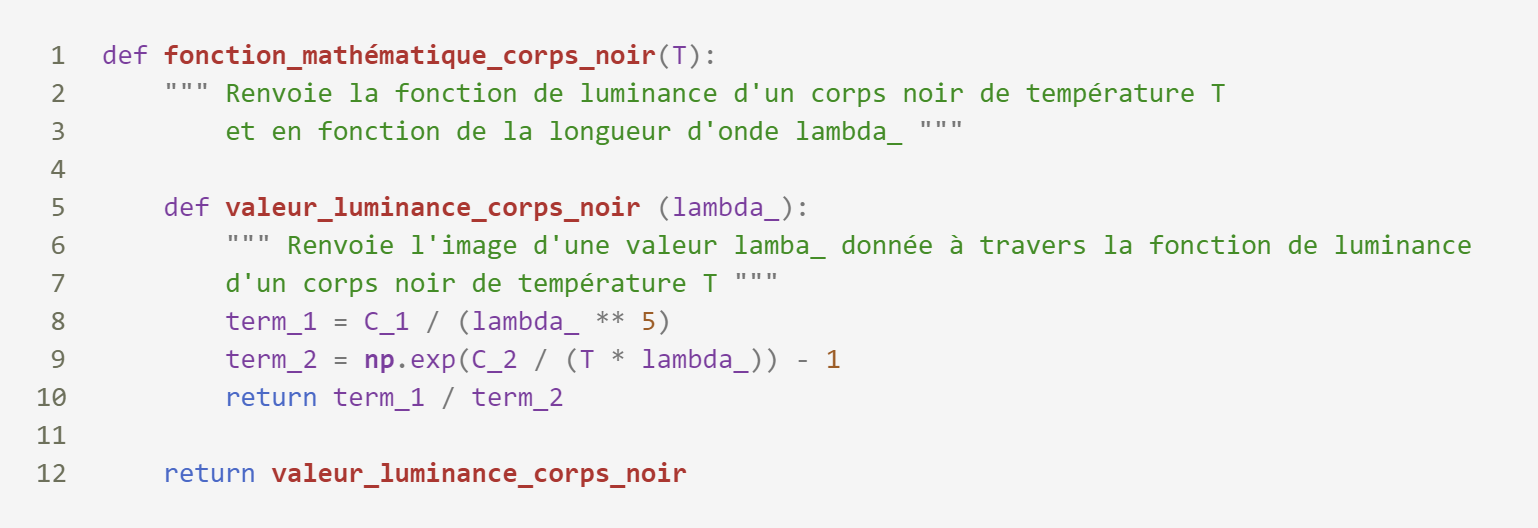
\includegraphics[scale=0.25]{Images/Code fonction luminance corps noir.png}
    \annexe{Fonction luminance corps noir}{Code de la fonction d'émittance d'un corps noir}
\end{center}

\begin{center}
    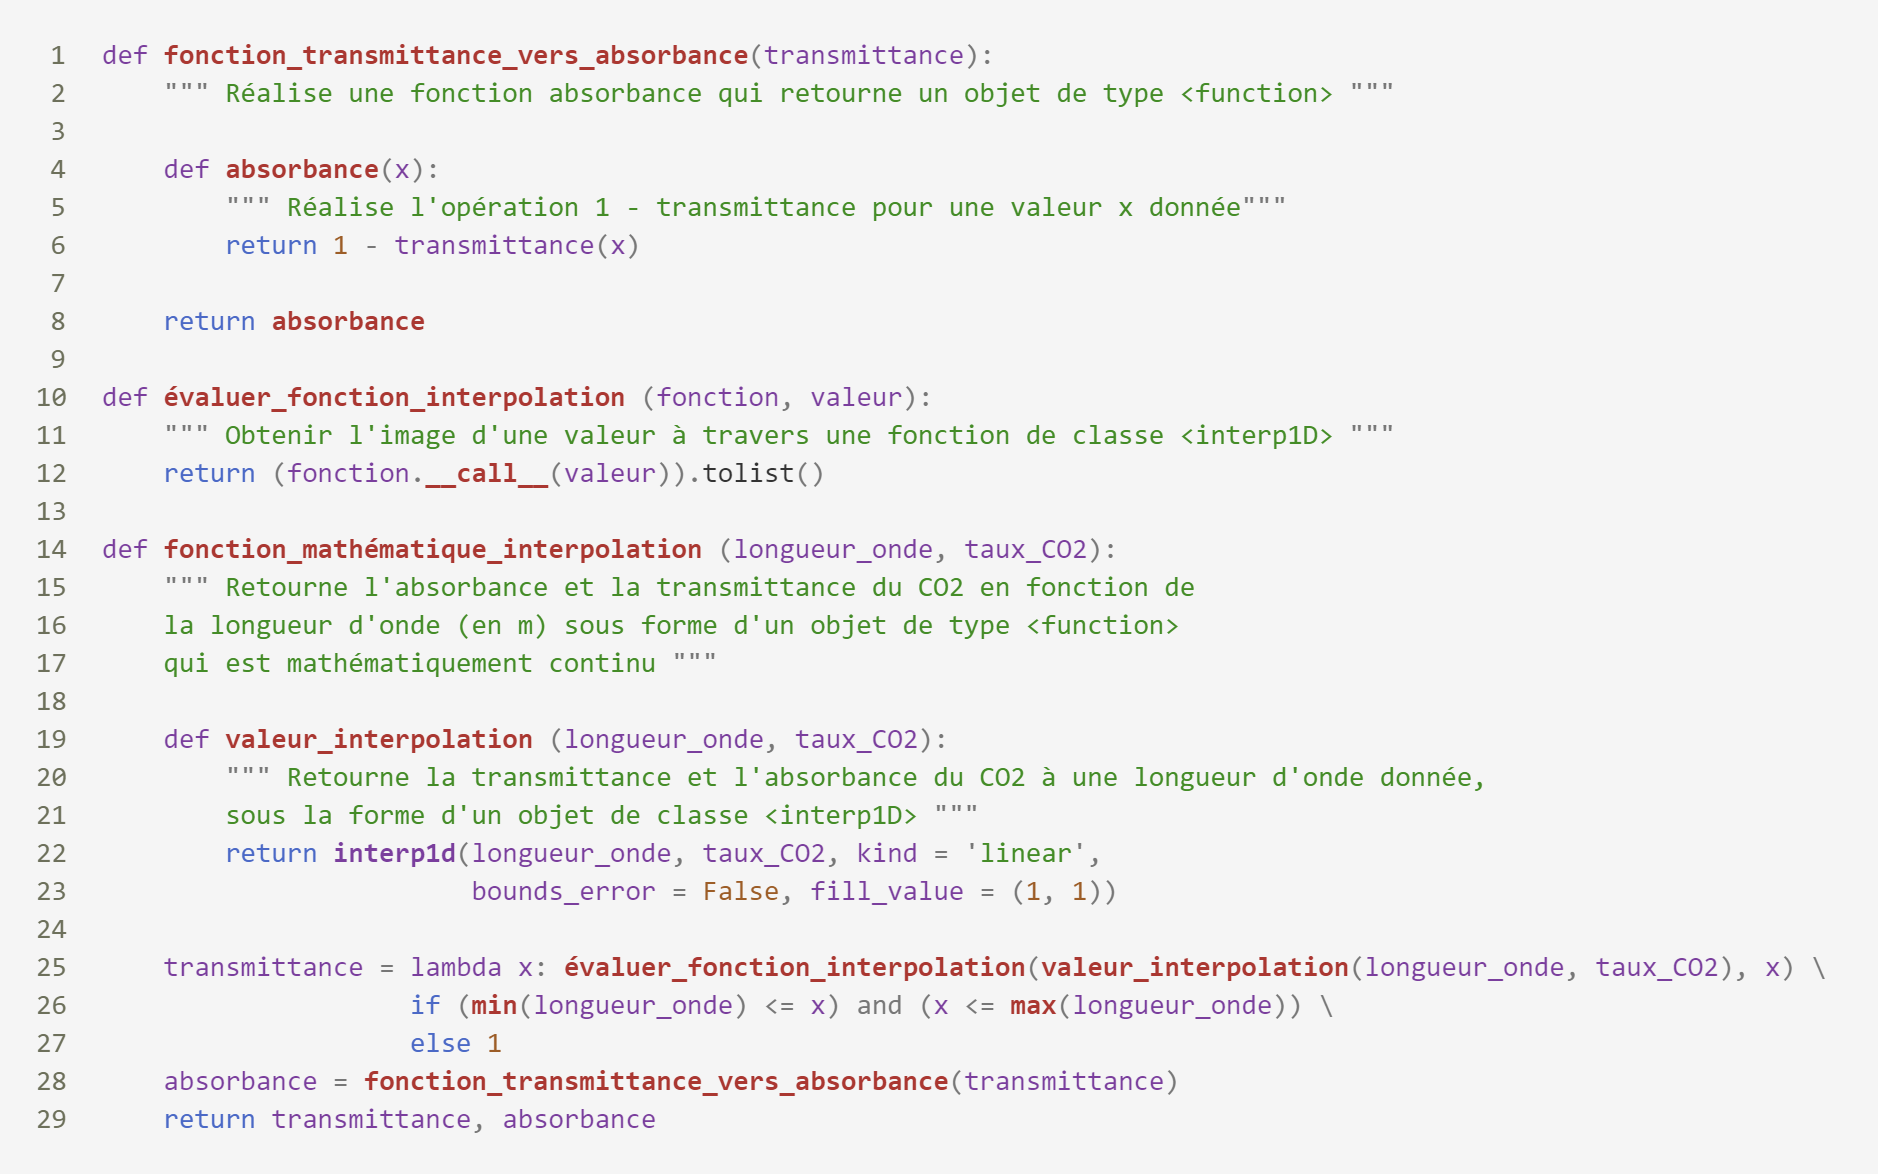
\includegraphics[scale=0.25]{Images/Interpolation.png}
    \annexe{Annexe Interpolation}{Fonctions d'interpolation et de prolongement par continuité}
\end{center}

\begin{center}
    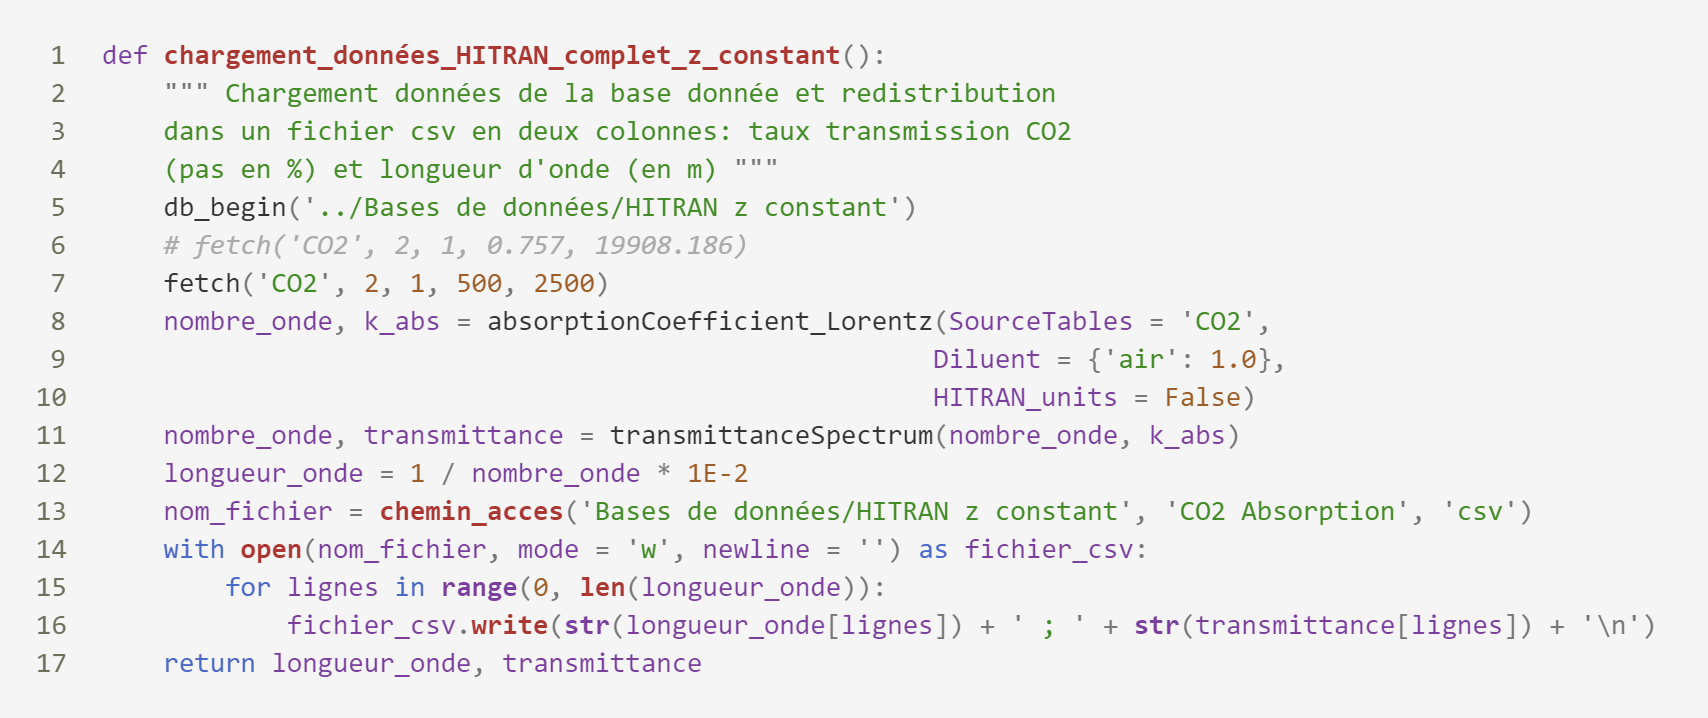
\includegraphics[scale=0.25]{Images/Hitran z constant.png}
    \annexe{Annexe Hitran z constant}{Fonction de récupération des données HITRAN modèle isotherme}
\end{center}

\begin{center}
    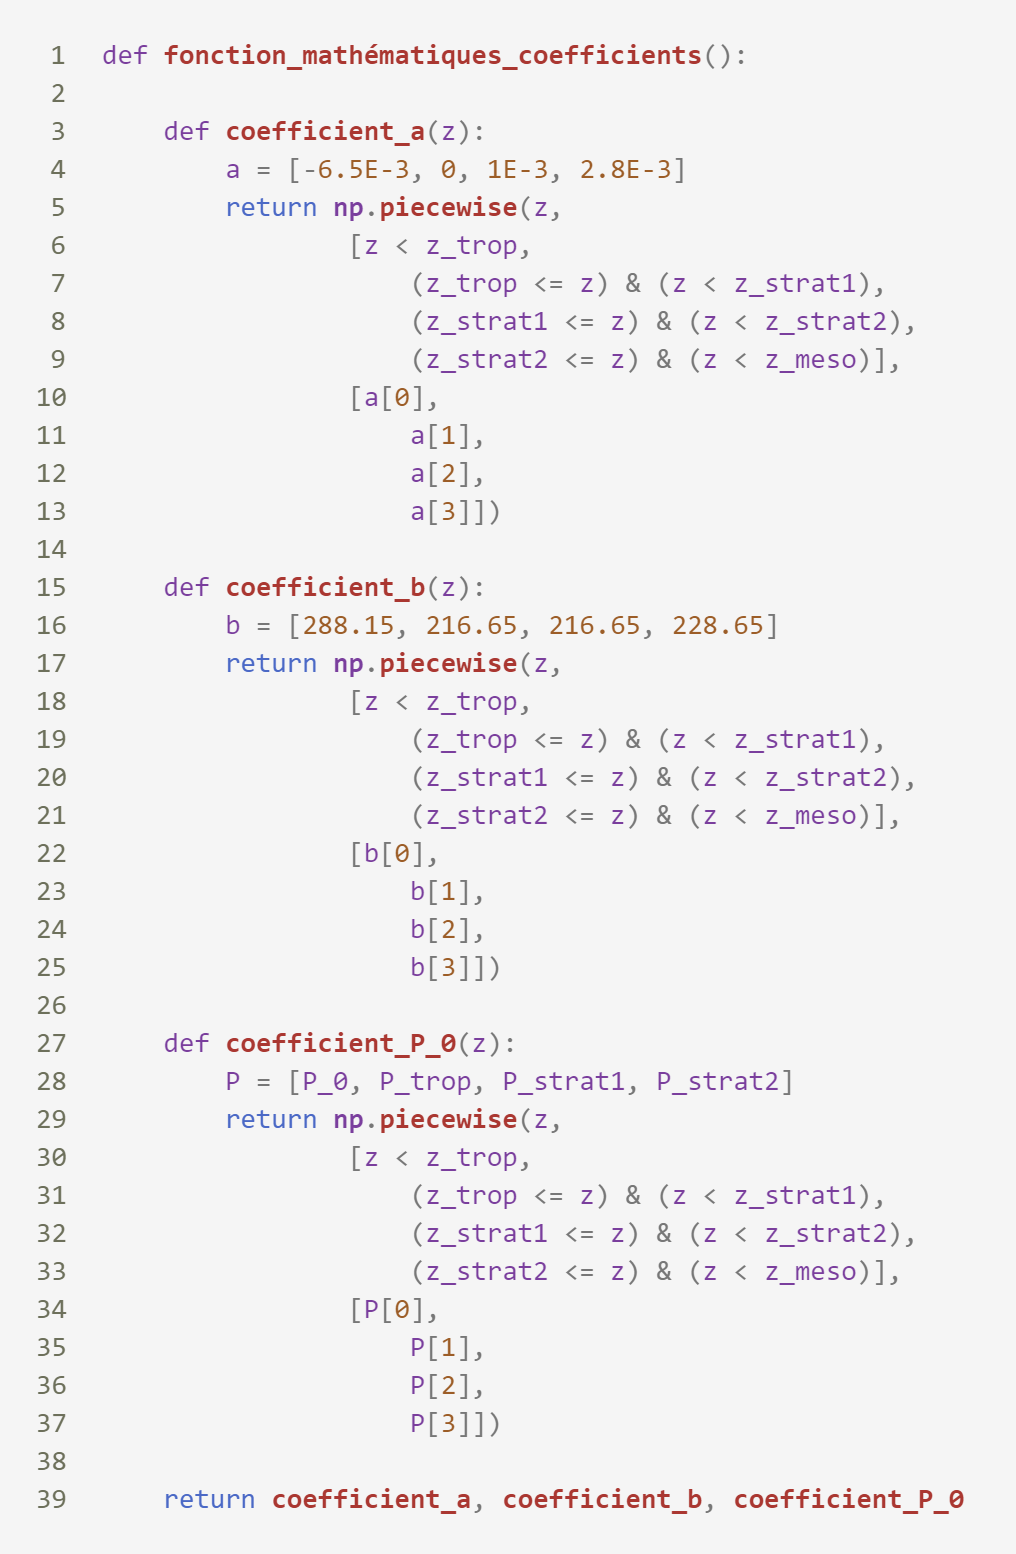
\includegraphics[scale=0.3]{Images/Fonction coefficients.png}
    \annexe{Annexe Fonction  coefficients}{Fonction définie par morceau de des divers coefficients}
\end{center}

\begin{center}
    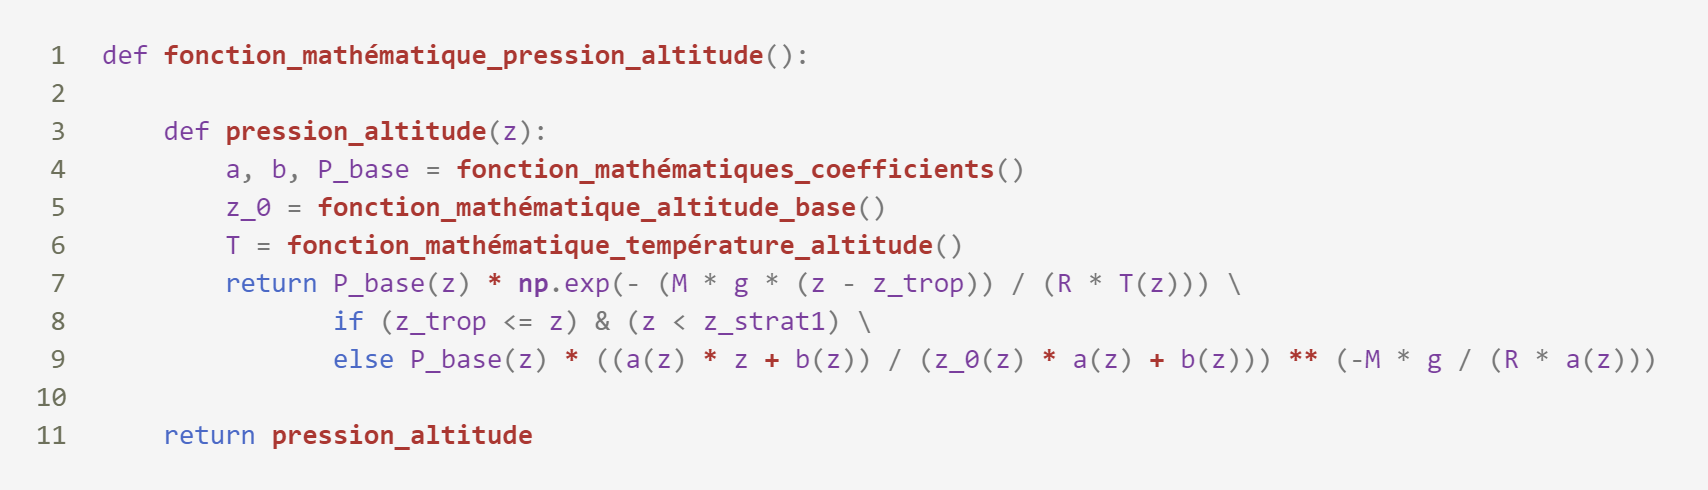
\includegraphics[scale=0.27]{Images/Fonction pression.png}
    \annexe{Annexe Fonction pression}{Fonction définie par morceau de la pression}
\end{center}

\begin{center}
    \includegraphics[scale=0.3]{Images/Fonction température.png}
    \annexe{Annexe Fonction température}{Fonction définie par morceau de la température}
\end{center}

\begin{center}
    \includegraphics[scale=0.4]{Images/Fonction densité particulaire volumique.png}
    \annexe{Annexe Fonction DPV}{Fonction définie par morceau de la densité particulaire volumique}
\end{center}

\end{document}